\documentclass[nobib,a4paper,oneside,openany]{tufte-book}

\hypersetup{colorlinks}% uncomment this line if you prefer colored hyperlinks (e.g., for onscreen viewing)

%%
% Book metadata
%\title{}
\author{Stefan F. Schouten}
\publisher{Publisher of This Book}

%%
% If they're installed, use Bergamo and Chantilly from www.fontsite.com.
% They're clones of Bembo and Gill Sans, respectively.
%\IfFileExists{bergamo.sty}{\usepackage[osf]{bergamo}}{}% Bembo
%\IfFileExists{chantill.sty}{\usepackage{chantill}}{}% Gill Sans

%\usepackage{microtype}

%%
% Just some sample text
\usepackage{lipsum}

%%
% For nicely typeset tabular material
\usepackage{booktabs}

%%
% For graphics / images
\usepackage{graphicx}
\setkeys{Gin}{width=\linewidth,totalheight=\textheight,keepaspectratio}
\graphicspath{{graphics/}}

% The fancyvrb package lets us customize the formatting of verbatim
% environments.  We use a slightly smaller font.
\usepackage{fancyvrb}
\fvset{fontsize=\normalsize}

% bib
\usepackage[
    style=authoryear,
    maxcitenames=2,
    backend=biber
]{biblatex}
\addbibresource{references.bib}


% ==== debugging stuff ===
\usepackage[disable]{todonotes}
%\usepackage{todonotes}
% ========================


\usepackage{glossaries}

\usepackage{marginfix}
\usepackage{placeins}


\usepackage{geometry}
\usepackage{float}

% ======= maths ==========
\usepackage{amsmath}
\usepackage{amssymb}
\usepackage{bm}
% ========================

% === prettier tables ====
\usepackage{booktabs}
\usepackage{multirow}

\usepackage{tablefootnote}

\usepackage{caption}
\usepackage{subcaption}
% ========================


% prettier urls
\newcommand\rurl[1]{%
  \href{http://#1}{\nolinkurl{#1}}%
}


% to mark as temporary
\newcommand{\tmp}[1]{{\color{red}{#1}}}

% bold vectors
\let\vec\mathbf

% prevent certain commands from showing up in a \nameref
\usepackage{etoolbox}
\makeatletter
\newcommand\@namedisablecommands{}
\newcommand{\addnamedisablecommand}[1]{%
  \g@addto@macro\@namedisablecommands{\renewcommand#1{}}%
  \pdfstringdefDisableCommands{\renewcommand#1{}}%
}
\AtBeginDocument{ 
  \patchcmd{\T@nameref}
  {\let\label\@gobble}
  {\let\label\@gobble\@namedisablecommands}
  {}{}
}
\makeatother

% citations
\DeclareCiteCommand{\citedoi}{
    \boolfalse{citetracker}%
    \boolfalse{pagetracker}%
    \usebibmacro{prenote}
}{%
    \iffieldundef{doi}{%
        \iffieldundef{url}{}{\printfield{url}}%
    }{\printfield{doi}}%
}{%
    \multicitedelim%
}{%
    \usebibmacro{postnote}%
}

\long\def\@stefan@tersefootcite[#1][#2]#3{%
    \sidenote[#1][#2]{\citefield{#3}[title]{title} \citedoi{#3}}%
}
\newcommand{\tersefootcite}{%
    \optparams{\@stefan@tersefootcite}{[][0pt]}%
}

\newcommand{\mycite}[2][0pt]{%
    \cite{#2}\tersefootcite[][#1]{#2}%
}
\newcommand{\mycitep}[2][0pt]{%
    \parencite{#2}\tersefootcite[][#1]{#2}%
}
\newcommand{\citep}[1]{\parencite{#1}}


% maths notations
\DeclareMathOperator*{\argmax}{arg\,max}
\DeclareMathOperator*{\argmin}{arg\,min}

\newcommand{\simpnt}{\overset{\textbf{.}}{=}}

%\newcommand{\simpnt}{\simeq\kern-0.96em{\cdot}\kern0.725em}
%\newcommand{\simpnt}{\overset{\raisebox{-1pt}{{.}}}{\simeq}}
%\newcommand{\simpnt}{\overset{\textbf{.}}{\simeq}}

%\newcommand{\simpnt}{\overset{.}{\sim}}
%\newcommand{\simpnt}{\sim \kern-0.87em{\boldsymbol{\cdot}}\kern0.725em}


% to create fixed-size paragraphs
\newcommand{\fixedpar}[1]{\par
   \def\x{\par\vskip-\prevgraf\baselineskip\vskip#1\baselineskip}%
   \bgroup\aftergroup\x\let\next=}



%%%%%%%%%%%%%%%%%%%%%%%%%%%%%%
%% v v v TUFTE MACROS v v v %%
%%%%%%%%%%%%%%%%%%%%%%%%%%%%%%

%%
% Prints argument within hanging parentheses (i.e., parentheses that take
% up no horizontal space).  Useful in tabular environments.
\newcommand{\hangp}[1]{\makebox[0pt][r]{(}#1\makebox[0pt][l]{)}}

%%
% Prints an asterisk that takes up no horizontal space.
% Useful in tabular environments.
\newcommand{\hangstar}{\makebox[0pt][l]{*}}

%%
% Prints a trailing space in a smart way.
\usepackage{xspace}

%%
% Some shortcuts for Tufte's book titles.  The lowercase commands will
% produce the initials of the book title in italics.  The all-caps commands
% will print out the full title of the book in italics.
\newcommand{\vdqi}{\textit{VDQI}\xspace}
\newcommand{\ei}{\textit{EI}\xspace}
\newcommand{\ve}{\textit{VE}\xspace}
\newcommand{\be}{\textit{BE}\xspace}
\newcommand{\VDQI}{\textit{The Visual Display of Quantitative Information}\xspace}
\newcommand{\EI}{\textit{Envisioning Information}\xspace}
\newcommand{\VE}{\textit{Visual Explanations}\xspace}
\newcommand{\BE}{\textit{Beautiful Evidence}\xspace}

\newcommand{\TL}{Tufte-\LaTeX\xspace}

% Prints the month name (e.g., January) and the year (e.g., 2008)
\newcommand{\monthyear}{%
  \ifcase\month\or January\or February\or March\or April\or May\or June\or
  July\or August\or September\or October\or November\or
  December\fi\space\number\year
}


% Prints an epigraph and speaker in sans serif, all-caps type.
\newcommand{\openepigraph}[2]{%
  %\sffamily\fontsize{14}{16}\selectfont
  \begin{fullwidth}
  \sffamily\large
  \begin{doublespace}
  \noindent\allcaps{#1}\\% epigraph
  \noindent\allcaps{#2}% author
  \end{doublespace}
  \end{fullwidth}
}

% Inserts a blank page
\newcommand{\blankpage}{\newpage\hbox{}\thispagestyle{empty}\newpage}

\usepackage{units}

% Typesets the font size, leading, and measure in the form of 10/12x26 pc.
\newcommand{\measure}[3]{#1/#2$\times$\unit[#3]{pc}}

% Macros for typesetting the documentation
\newcommand{\hlred}[1]{\textcolor{Maroon}{#1}}% prints in red
\newcommand{\hangleft}[1]{\makebox[0pt][r]{#1}}
\newcommand{\hairsp}{\hspace{1pt}}% hair space
\newcommand{\hquad}{\hskip0.5em\relax}% half quad space
\newcommand{\TODO}{\textcolor{red}{\bf TODO!}\xspace}
\newcommand{\ie}{\textit{i.\hairsp{}e.}\xspace}
\newcommand{\eg}{\textit{e.\hairsp{}g.}\xspace}
\newcommand{\na}{\quad--}% used in tables for N/A cells
\providecommand{\XeLaTeX}{X\lower.5ex\hbox{\kern-0.15em\reflectbox{E}}\kern-0.1em\LaTeX}
\newcommand{\tXeLaTeX}{\XeLaTeX\index{XeLaTeX@\protect\XeLaTeX}}
% \index{\texttt{\textbackslash xyz}@\hangleft{\texttt{\textbackslash}}\texttt{xyz}}
\newcommand{\tuftebs}{\symbol{'134}}% a backslash in tt type in OT1/T1
\newcommand{\doccmdnoindex}[2][]{\texttt{\tuftebs#2}}% command name -- adds backslash automatically (and doesn't add cmd to the index)
\newcommand{\doccmddef}[2][]{%
  \hlred{\texttt{\tuftebs#2}}\label{cmd:#2}%
  \ifthenelse{\isempty{#1}}%
    {% add the command to the index
      \index{#2 command@\protect\hangleft{\texttt{\tuftebs}}\texttt{#2}}% command name
    }%
    {% add the command and package to the index
      \index{#2 command@\protect\hangleft{\texttt{\tuftebs}}\texttt{#2} (\texttt{#1} package)}% command name
      \index{#1 package@\texttt{#1} package}\index{packages!#1@\texttt{#1}}% package name
    }%
}% command name -- adds backslash automatically
\newcommand{\doccmd}[2][]{%
  \texttt{\tuftebs#2}%
  \ifthenelse{\isempty{#1}}%
    {% add the command to the index
      \index{#2 command@\protect\hangleft{\texttt{\tuftebs}}\texttt{#2}}% command name
    }%
    {% add the command and package to the index
      \index{#2 command@\protect\hangleft{\texttt{\tuftebs}}\texttt{#2} (\texttt{#1} package)}% command name
      \index{#1 package@\texttt{#1} package}\index{packages!#1@\texttt{#1}}% package name
    }%
}% command name -- adds backslash automatically
\newcommand{\docopt}[1]{\ensuremath{\langle}\textrm{\textit{#1}}\ensuremath{\rangle}}% optional command argument
\newcommand{\docarg}[1]{\textrm{\textit{#1}}}% (required) command argument
\newenvironment{docspec}{\begin{quotation}\ttfamily\parskip0pt\parindent0pt\ignorespaces}{\end{quotation}}% command specification environment
\newcommand{\docenv}[1]{\texttt{#1}\index{#1 environment@\texttt{#1} environment}\index{environments!#1@\texttt{#1}}}% environment name
\newcommand{\docenvdef}[1]{\hlred{\texttt{#1}}\label{env:#1}\index{#1 environment@\texttt{#1} environment}\index{environments!#1@\texttt{#1}}}% environment name
\newcommand{\docpkg}[1]{\texttt{#1}\index{#1 package@\texttt{#1} package}\index{packages!#1@\texttt{#1}}}% package name
\newcommand{\doccls}[1]{\texttt{#1}}% document class name
\newcommand{\docclsopt}[1]{\texttt{#1}\index{#1 class option@\texttt{#1} class option}\index{class options!#1@\texttt{#1}}}% document class option name
\newcommand{\docclsoptdef}[1]{\hlred{\texttt{#1}}\label{clsopt:#1}\index{#1 class option@\texttt{#1} class option}\index{class options!#1@\texttt{#1}}}% document class option name defined
\newcommand{\docmsg}[2]{\bigskip\begin{fullwidth}\noindent\ttfamily#1\end{fullwidth}\medskip\par\noindent#2}
\newcommand{\docfilehook}[2]{\texttt{#1}\index{file hooks!#2}\index{#1@\texttt{#1}}}
\newcommand{\doccounter}[1]{\texttt{#1}\index{#1 counter@\texttt{#1} counter}}
\newglossaryentry{linkprediction}
{
    name=Link Prediction,
    description={}
}

\newglossaryentry{kge}
{
    name=Knowledge Graph Embedding,
    plural=Knowledge Graph Embeddings,
    description={}
}




% Generates the index
\usepackage{makeidx}
\makeindex

% set section numbering depth
\setcounter{secnumdepth}{1}

% remove \todo from \nameref
\addnamedisablecommand{\todo[2][]}
% remove \cite from \nameref
\addnamedisablecommand{\cite[2][]}


%%%%%%%%%%%%%%%%%%%%%%%%%%%%%%
%%  v v v  DOCUMENT  v v v  %%
%%%%%%%%%%%%%%%%%%%%%%%%%%%%%%

\begin{document}

% Front matter
\frontmatter
\begingroup 

\let\cleardoublepage\relax
\let\clearpage\relax

% blank page
%\blankpage
%\begin{fullwidth}
%\newpage\thispagestyle{empty}
%\end{fullwidth}

% epigraphs
%\newpage\thispagestyle{empty}
%\tmp{
%    \openepigraph{%
%        The public is more familiar with bad design than good design.
%        It is, in effect, conditioned to prefer bad design, 
%        because that is what it lives with. 
%        The new becomes threatening, the old reassuring.
%    }{Paul Rand%, {\itshape Design, Form, and Chaos}
%    }
%}
%\vfill
%\tmp{
%\openepigraph{%
%        A designer knows that he has achieved perfection 
%        not when there is nothing left to add, 
%        but when there is nothing left to take away.
%    }{Antoine de Saint-Exup\'{e}ry}
%}
%\vfill
%\tmp{
%    \openepigraph{%
%    \ldots the designer of a new system must not only be the implementor and the first 
%        large-scale user; the designer should also write the first user manual\ldots 
%        If I had not participated fully in all these activities, 
%        literally hundreds of improvements would never have been made, 
%        because I would never have thought of them or perceived 
%        why they were important.
%    }{Donald E. Knuth}
%}


% full title page
%\maketitle
\newgeometry{margin=2cm}

\begin{titlepage}

\newcommand{\HRule}{\rule{\linewidth}{0.5mm}} % Defines a new command for the horizontal lines, change thickness here

\center % Center everything on the page

 
%----------------------------------------------------------------------------------------
%	HEADING SECTIONS
%----------------------------------------------------------------------------------------


\includegraphics[width=\linewidth]{uva_logo.jpg}\\[2.5cm]

\textsc{\Large MSc Artificial Intelligence}\\[0.2cm]

\textsc{\Large Master Thesis}\\[0.5cm] 


%----------------------------------------------------------------------------------------
%	TITLE SECTION
%----------------------------------------------------------------------------------------

\HRule \\[0.4cm]

% Title of your document
%{ \huge \bfseries \tmp{Your Title that will take\\ Two Lines} }\\[0.4cm] 
{ \huge \bfseries {Incorporating Semantics\\ in Knowledge Graph Embeddings} }\\[0.4cm] 
\HRule \\[0.5cm]

 
%----------------------------------------------------------------------------------------
%	AUTHOR SECTION
%----------------------------------------------------------------------------------------

by\\[0.2cm]

\textsc{\Large Stefan F. Schouten}\\[0.2cm] %you name

{12808113}\\[1cm]


%----------------------------------------------------------------------------------------
%	DATE SECTION
%----------------------------------------------------------------------------------------

{\Large \today}\\[1cm] % Date, change the \today to a set date if you want to be precise



%----------------------------------------------------------------------------------------

48 ECTS\\ %

October 2020 - July 2021\\[1cm]%



%----------------------------------------------------------------------------------------
%	COMMITTEE SECTION
%----------------------------------------------------------------------------------------

\begin{minipage}[t]{0.7\textwidth}
    \begin{flushleft} \large
        \emph{Supervisors:} \\
        Thiviyan \textsc{Thanapalasingam} MSc \\
        Daniel \textsc{Daza} MSc \\
    \end{flushleft}
\end{minipage}

~

\begin{minipage}[t]{0.7\textwidth}
    \begin{flushright} \large
        \emph{Assessor:} \\
        Dr. Paul \textsc{Groth}\\
    \end{flushright}
\end{minipage}\\[2cm]



%----------------------------------------------------------------------------------------
%	LOGO SECTION
%----------------------------------------------------------------------------------------


%\framebox{\rule{0pt}{2.5cm}\rule{2.5cm}{0pt}}\\[0.5cm]

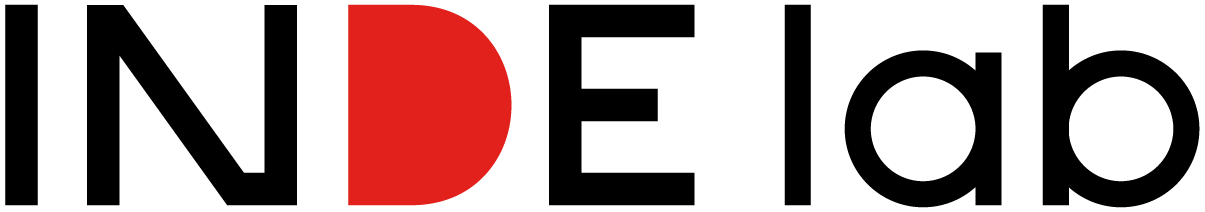
\includegraphics[width=5cm]{indelab_logo.png}\\ % Include a department/university logo - this will require the graphicx package

\textsc{\large INtelligent Data Engineering Lab}\\[1.0cm] % 


%----------------------------------------------------------------------------------------


\vfill % Fill the rest of the page with whitespace

\end{titlepage}

\restoregeometry

% abstract
\newpage
\begin{fullwidth}
    \center
    \thispagestyle{empty}
    \begin{minipage}[h]{0.7\linewidth}
        \vspace{5cm}
        
        \center
        \textsc{\Large \textbf{Abstract}}\\[0.5em]
        
        \justify
        % MOTIVATION
        \glspl*{kge} (KGEs) aim to represent the entities and relations within a Knowledge Graph using continuous vector representations. This allows them to be utilized more easily for tasks such as Link Prediction, Relation Extraction, and Question Answering.
        Commonly, these embeddings focus on representing the structure of the Knowledge Graph, but incorporating semantics may increase their utility.
        % CORE OF METHOD
        We compare several methods that incorporate an abundantly available form of semantics: type-information.
        We include an existing method, TransT, as well as new methods that either construct entity-embeddings from type-embeddings, or model type-distributions over entity-embeddings.
        We perform extensive hyper-parameter searches in order to compare the performance of these methods when applied to the Link Prediction task.
        % MAIN RESULT
        % surprisingly high performance 
        We observe up to 261\% increase of MRR against a TransE baseline for a class of methods that learned to represent each entity by one of its types, using that type's embedding as the entity's embedding. Other methods result in a modest increase in performance relative to their non-semantic baseline.
        % TAKEAWAY
        While it remains challenging to incorporate type-information such that it may benefit more than just Link Prediction, the high performance we observe shows there is great potential in its utilization.
    \end{minipage}
\end{fullwidth}

% copyright page
%\newpage
%\begin{fullwidth}
%    ~\vfill
%    \thispagestyle{empty}
%    \setlength{\parindent}{0pt}
%    \setlength{\parskip}{\baselineskip}
%    Copyright \copyright\ \the\year\ \thanklessauthor
%    
%    %\par\smallcaps{Published by \thanklesspublisher}
%    \tmp{
%    \par\smallcaps{tufte-latex.googlecode.com}
%    }
%    \tmp{
%    \par Licensed under the Apache License, Version 2.0 (the ``License''); you may not
%    use this file except in compliance with the License. You may obtain a copy
%    of the License at \url{http://www.apache.org/licenses/LICENSE-2.0}. Unless
%    required by applicable law or agreed to in writing, software distributed
%    under the License is distributed on an \smallcaps{``AS IS'' BASIS, WITHOUT
%    WARRANTIES OR CONDITIONS OF ANY KIND}, either express or implied. See the
%    License for the specific language governing permissions and limitations
%    under the License.\index{license}
%    }
    %\par\textit{First printing, \monthyear}
%\end{fullwidth}

% contents
\newpage

\setcounter{tocdepth}{1}
\tableofcontents
\newpage

\listoffigures
\newpage

\listoftables

% preface
\newpage
\chapter{Preface}

The first time I became interested in Knowledge Graphs was during my bachelor's thesis project.
During the project we developed a prototype for the automated summarization of medical consultation dialogues. The architecture we were tasked with implementing envisioned a knowledge graph (with prespecified ontology) at the center. Facts from the dialogue would first be extracted and stored in the knowledge graph, and then the relevant part of the knowledge graph would be used to generate a summary.

Under some naive assumptions we managed to implement this well enough for a proof of concept. But since then I've been fascinated by the possibility of taking advantage of recent advances in Deep Learning to perform this kind of knowledge extraction from natural language.
What motivated me to choose the topic of this thesis was that the inclusion of semantics (both those represented in an ontology, and those from natural languages) in Knowledge Graph Embeddings seems vital for them to be used in this type of knowledge extraction. 
\\[0.5em]

\noindent I would like to thank my supervisors Thiviyan Thanapalasingam and Daniel Daza for their frequent encouragement and reassurance, as well as their excellent advice throughout this project.
\\[0.5cm]

\noindent
Stefan F. Schouten
\\[0.5cm]
 
\noindent
Gouda, \today

%%
% Start the main matter (normal chapters)
\endgroup
\mainmatter

\chapter{Introduction}
\label{ch:introduction}
% Make the case for Knowledge Graphs in general.
% Motivate the use of them in combination with machine/deep learning.
% Sketch overview of research so far
% point out that only limited research has been done that tries to incorporate semantics
% talk about what makes the inclusion of semantics valuable
% move into talking about what we investigate now
% give research questions ( / hypotheses ?)

% \todo[inline,caption={}]{
% \begin{itemize}
%     \item Capture attention, foreshadow main objective of thesis.
%     \item General introduction into Knowledge Graphs.
%     \item Maybe some historical factoids, motivation behind them, etc.
% \end{itemize}
% }

Knowledge Graphs represent (real-world) information using a graph-based structure. 
They are used to represent both domain-specific and general information. Nodes in the graph represent entities, whereas the edges between nodes represent a various kinds of relations that exist between two entities.

Knowledge Graphs are already critical to the operation of large tech companies such as Microsoft, Google and Facebook, where they are used to integrate and manage data from diverse sources at a large scale \mycitep{noy_industry-scale_2019}. 
%
Knowledge graphs are also strongly related to concepts in the Semantic Web, the effort to make information on the Internet machine-readable \mycitep{Paulheim2017}. 

Despite their widespread use, knowledge graphs are generally not complete, entities that should be connected by a given relation are often not. Within the field of Artificial Intelligence, research is conducted into a task known as Knowledge Graph Completion. That task's objective is to identify missing facts which should be added to the knowledge graph. When this task is performed primarily using information found within the knowledge graph itself it is also referred to as Link Prediction \mycitep{rossi_knowledge_2021}.

To perform tasks like Link Prediction the Knowledge Graph can be embedded. Traditionally only the Knowledge Graph's syntactical information is incorporated in such an embedding. While this information alone can already model the Knowledge Graph quite well, this thesis will explore ways of also incorporating semantics to improve their performance.

%\todo[inline]{Answer: what is missing in existing link prediction models, what motivated the research, what are we trying to explore}

\paragraph{}\noindent
In this chapter we will introduce the relevant notation, explain what task this thesis will focus on, and finally we will formulate the exact research question.

\subsection*{Knowledge Graph}
%
% Background for notation, not for reader, but so I don't forget.
% Notation should have mapping into proper probability theory.
% Sample space (\Omega) is the power set of \mathcal{D}, 2^\mathcal{D}.
% 
A Knowledge Graph consists of a set of entities $\mathcal{E} = \{ e_{i} \}$, a set of relations $\mathcal{R} = \{ r_{j} \}$, and a set of facts $\mathcal{D}^+$:
\marginnote{Note that $\mathcal{D}^+$ only contains observations $X_k = True$. What we assume about $X$ for the triples that are not in $D^+$ determines if we operate under an open- or closed-world assumption. Under an open-world assumption we consider the other $X$'s to be unknown, under a closed-world assumption we consider them to be $False$.}
\begin{equation}
    \mathcal{D}^+ \subseteq \mathcal{D} = \mathcal{E} \times \mathcal{R} \times \mathcal{E} =  \{ (e_{head}, r, e_{tail})^{(k)} \} = \{ (h, r, t)^{(k)} \};
\end{equation}
which determines which entities are related by what relations. 
The set $\mathcal{D}^+$ can also be considered as a set of observations of the Boolean random variable:
\begin{align}
    & X^{(k)} & &\text{truth value of triple $k$.} 
% elements of $2^\mathcal{D}$ that have $(h, r, t)^{(k)}$
\end{align}
\marginnote[2em]{Here the small $x^{(k)}$ is a value that the random variable $X^{(k)}$ might take (True or False). Throughout this document $\Gamma | a$ is short for $\Gamma | A = a$.}
%
%It is often useful to think of the elements of Knowledge Graphs as being (conditional) random variables.
We can also consider the components of the triples to be random variables. For an arbitrary triple with index $k'$ we might consider the following conditional random variables:
\begin{equation} \label{eq:ex_cond_rv1}
    H^{(k')} | x^{(k')}; \hspace{2em} R^{(k')} | x^{(k')}; \hspace{2em} T^{(k')} | x^{(k')} .
% elements of $2^\mathcal{D}$ that 
% {H = h | X = x} = { D^+ \elem 2^\mathcal{D} :  }
\end{equation}
To avoid notational overload we drop the index whenever we refer to an arbitrary triple, giving simply:
\begin{equation} \label{eq:ex_cond_rv2}
    H | x; \hspace{2em} R | x; \hspace{2em} T | x .
\end{equation}
Their distribution says something about the likelihood of entities and relations being the Head, Relation, or Tail within a triple with truth value $x$. 
Here $H$, $T$ and $R$ are categorical random variables with $\mathcal{E}$ and $\mathcal{R}$ as their support respectively. 
%This also means that when we speak of the values $h^{(k)}, r^{(k)}, t^{(k)}$ that these random variables might take are mere references to the elements of $\mathcal{E}$ and $\mathcal{R}$.
%And $h^{(k)}, r^{(k)}, t^{(k)}$ are merely references to the entities $e \in \mathcal{E}$ and relations $r \in \mathcal{R}$ that occur in the $k$-th triple in $\mathcal{D}$.



%%%%%%%%%%%%%%%%%%%%
%%   EMBEDDINGS   %%
%%%%%%%%%%%%%%%%%%%%
\subsection*{Knowledge Graph Embedding (KGE)}
% goal of embedding them (use in machine learning)
% 
% traditionally to encode structural information only

When we learn an embedding we associate symbols with continuous vector representations. We are concerned with learning such representations for the entities and relations in our Knowledge Graph. We wish to do so in order to use machine learning techniques such as Deep Learning. These techniques can then be used for a range of applications such as Link Prediction, Entity Classification, Relation Extraction, and Question Answering \mycitep{kge_survey_2017}.

When tasked with learning a \gls*{kge}, we (implicitly) postulate additional unobserved multidimensional random variables\sidenote[][2em]{To avoid notational overload once more, we refer to these as simply $\vec{H}, \vec{R}, \vec{T}$ whenever we mean an arbitrary triple, or as $ \vec{H}^{(k)}, \vec{R}^{(k)}, \vec{T}^{(k)}$ when we mean a specific triple's embedding.} for arbitrary triple $k'$:
\begin{align}
\vec{H}^{(k')} | H^{(k')} = h^{(k')} ; 
\hspace{1.5em} 
\vec{R}^{(k')} | R^{(k')} = r^{(k')} ;
\hspace{1.5em} 
\vec{T}^{(k')} | T^{(k')} = t^{(k')} .
\end{align}
In other words, we imagine that the truth value for each possible triple was sampled from a distribution $p(x|\vec{h}, \vec{r}, \vec{t})$; where $\vec{h}, \vec{r},$ and $\vec{t}$ were in turn sampled from unknown posterior $p(\vec{h}, \vec{r}, \vec{t}|h,r,t)$. We are interested in approximating that posterior, thereby also gaining access to samples $(\vec{h}, \vec{r}, \vec{t})$ which we can use as the embeddings we seek.
%
%\marginnote[-7em]{While the latent embeddings $\vec{E}$ and $\vec{R}$ are continuous random variables with $\mathbb{R}^{D}$ as their support, the variables $E$ and $R$ are categorical, and $X$ is boolean.}
%
%\marginnote{There are no independent random variables $\vec{H}^{(k)}, \vec{R}^{(k)}, \vec{T}^{(k)}$, they are merely references to one of the random variables $\vec{E}_i, \vec{R}_i$. Example: $\vec{H}^{(k)} = \vec{E}_{h(k)}$. }
%
Because we often model the distribution of the embeddings without considering the position of the entities in a triple, we also define:
\marginnote{That is to say, we model the posterior $p(\vec{h}, \vec{r}, \vec{t}|h,r,t)$ as $q_e(\vec{h}|h) q_r(\vec{r}|r) q_e(\vec{t}|t)$, i.e. forcing ourselves to use the same approximate posterior for $\vec{H}$ and $\vec{T}$.}
\begin{align}
    \vec{E}_i :=\ \vec{H}|H\!=\!e_i\ =\ \vec{T}|T\!=\!e_i % H = e_i \lor T = e_i; 
    \hspace{1.5em} \text{and} \hspace{1.5em}
    \vec{R}_j :=\ \vec{R}|R\!=\!r_j .
\end{align}

%Further, we also define the functions $h(k), r(k), t(k)$ as mappings from the index of a fact $(h,r,t)^{(k)}$ to: the index $i$ of the entity $e_i$ being referenced by $h$ or $t$; or the index $j$ of the relation $r_j$ being referenced by $r$.

When we make modeling decisions we make assumptions about how these random variables are distributed.
For this we use the following type of notation:
\begin{align}
    \vec{E}_i|\theta_i &\sim \text{Distribution}(f(\theta_i));
%\end{align}
\intertext{
where $\theta$ are model parameters.
Often Knowledge Graph Embeddings are not modeled as a distribution, but are modeled as point estimates. We denote this as follows:
}
%\begin{align}
    \vec{E}_i|\theta_i &\simpnt f(\theta_i);
\end{align}
that is to say the embeddings come from a deterministic function.

\subsection*{Semantic Information}
Frequently Knowledge Graph Embeddings are learned based only on structural (syntactical) information \mycitep{kge_survey_2017}, i.e. which entities are connected by what relations. But the underlying assumption, that the truth value of possible triples can be inferred from syntactical information only, is rather simplifying. 
The syntactical information might allow us to notice that when an entities connect by relation $r1$ to entity $a$, they often also connect by relation $r2$ to entity $b$. But we are never able to utilize other ways entities might be similar. 
There are a few distinct sources of semantic information we could use to improve upon this.
\begin{itemize}
    \item Often we know Natural Language names of the entities in the Knowledge Graph. These can be seen as a bridge to those languages, this could allow us to utilize models of the semantics of those languages for the Knowledge Graph as well.
    \item Information of how entities appear (look, sound, behave, etc.) in the real world could help with \textit{inferring} the semantics, since the real world is what we are trying to describe.
    \item Finally, the entities and relation-types in a Knowledge Graph come from our understanding of the world. One way to improve, is to describe more of that understanding manually by recording semantics in the form of an ontology. 
\end{itemize}
It is the latter that will be the focus of this thesis.

\paragraph{Including Ontological Information.} 
The most prevalent kind of ontological information are groupings of entities into classes.
For example, we might have access to a set of entity classes $\mathcal{C} = \{ c_s \}$. With corresponding observed random variable:
\begin{align}
&    C_{i,s} := C|e_i, c_s    &  &\text{whether entity $i$ is of type (or class) $c_s$.}
\end{align}
These entity classes are essentially categories or \textbf{types} of entities, for example the entity `Stefan' could be part of the `Person' type. When including this information in the embedding process we hope that the types an entity falls under are predictive of the truth value of a triple (for example because certain relations generally exist only between entities of certain types).


Other kinds of ontological information include \mycitep{hitzler_owl_2012}: %
\begin{itemize} \setlength\itemsep{0em}
    \item restrictions, for example on the entity types between which certain relations can exist;
    \item entity-type and relation hierarchies, for example a `hasCar' relation could be a specific kind of `hasProperty' relation;
    \item characteristics of relations, for example that a relation is symmetrical, i.e. if (h,r,t) is true then (t,r,h) is also true.
\end{itemize}

Previous work (\mycite{hao2019joie}; \mycite{zhou2020jeci}; \mycite{wang2020jeci})
has investigated also embedding the entity-types. 
One approach is to embed these types in the same space as the entities. 
In this case we are effectively learning an additional distribution of entity-representations, the difference is that this one is conditioned on the type(s), e.g. $p_i(\vec{e}_i|c_{i,1} \dots c_{i,n_c})$. 
Alternatively, entity-classes can be embedded in a separate space.
In both cases related ontological information, like a class hierarchy could also be incorporated.

% \paragraph{}
% Another kind of semantic information comes in the form of text. We frequently refer to entities and entity-classes by their English name, entities are often associated with a proper noun (`Stefan') and entity classes with a common noun (`person'). 
% For relations there is often some verb involved, we already saw the example `hasProperty', but we would normally use `owns' to express such a relation. 
% There are datasets that include either natural language descriptions of entities/relations; or even natural language assertions of given facts (triples). Information like this could be used to regularize training for the link prediction task, but is especially interesting when we are interested in extraction of entities and/or links from text.

%\begin{align}
%&    M^{(k)}_u             &  &\text{$u$-th symbol (word/character) in mention of $k$-th fact.}
%\end{align}
% \paragraph{}
% In principle there are many more kinds of semantic information. For example we might have visual (images, video, diagrams, etc.) information depicting entities or a state of affairs that implicitly asserts a given fact. Generally for each medium, one can imagine the existence of either assertions of fact, or descriptions of entities and/or relations. But in practice we do not see many (if any\todo{find out}) datasets with information of a kind other than ontological or textual.


\subsection*{Research Question}
Our concern is with `Incorporating semantics in knowledge graph embeddings'. We choose to focus primarily on the incorporation of type-information to improve Link Prediction performance.
Thus we ask the following research question: \\ 
\textit{(\textbf{RQ1})}
To what extent can type-information improve link-prediction performance? And,
\textit{(\textbf{RQ2})}
what method of incorporating the type-information is most effective?

To answer this question we will first review existing methods in the literature on this topic in Chapter \ref{ch:literature_review}. 
In Chapter \ref{ch:methodology} we will describe what methods for incorporating type-information we will investigate.
Chapter \ref{ch:experiments} will describe the experiments, as well as present and analyze the results. 
Finally, in Chapter \ref{ch:conclusion} we will discuss our findings, and answer the research questions.

\paragraph{}\noindent
We find that type-information is highly informative, and when used on its own, can outperform KGEs that do not use types at all. The difficulty is in incorporating the type-information in a KGE along with the other (entity-level) information, such that it has higher Link Prediction performance, and is still suitable for the same use cases (such as entity classification, question answering, etc.).



%\todo[inline]{Summarize contributions, findings. Outline of thesis with each chapter's content.}


% % MOTIVATION
% \glspl*{kge} (KGEs) aim to represent the entities and relations within a Knowledge Graph using continuous vector representations. This allows them to be utilized more easily for tasks such as Link Prediction, Relation Extraction, and Question Answering.
% Commonly, these embeddings focus on representing the structure of the Knowledge Graph, but incorporating semantics may increase their utility.
% % CORE OF METHOD
% We compare several methods that incorporate an abundantly available form of semantics: type-information.
% %These methods use a variety of ways to include the type-information, viewing them either as sets of entities with informative statistics, or as objects to be embedded along with the entities and relations.
% We include an existing method TransT, as well as new methods that either construct entity-embeddings from type-embeddings, or model type-distributions over entity-embeddings.
% We perform extensive hyper-parameter searches in order to compare the performance of these methods when applied to the Link Prediction task.
% % MAIN RESULT
% We observe surprisingly high performance for a class of methods that learned to represent each entity by one of its types, using that type's embedding as the entity's embedding. Other methods result in a modest increase in performance relative to their non-semantic baseline.
% % TAKEAWAY
% While it remains challenging to incorporate type-information such that it may benefit more than just Link Prediction, the high performance we observe shows there is great potential in its utilization. 
\chapter{Literature Review}
\label{ch:literature_review}
% General knowledge graph embedding papers: TransE, DistMult?
% These should be discussed to a point that it is clear what the widespread approaches 
% to this problem look like.
% Then move into papers that include semantics (type / text / visual? / ) 

% Discussion of a paper (from Zobel):
%  - In short: contribution to the field, limitations, and the questions that they leave open.
%  - Briefly summarize each paper’s contribution and the evidence used to support the claims.
%  - Note any shortcomings or features that are of interest.
%  - For your own reference, note how the work might have been done better.
%  - For the early versions: think of the writing as a letter to your future self

This chapter will provide an overview of relevant literature. It will start with a few generally applicable Knowledge Graph Embedding (KGE) methods, followed by recent methods that incorporate type-information.

\section{General KGE Methods}

Methods that attempt to incorporate semantics generally do so by modifying existing KGE methods. This section briefly describes some of these existing methods to provide the necessary background for the methods that follow in the rest of the chapter.

A recent survey \mycitep{rossi_knowledge_2021} divides KGE methods used for Link Prediction into three groups: tensor decomposition models, geometric models, and deep learning models. 
They differ from each other by the way that they calculate scores by which to rank triples on their likelihood of being true. 

\begin{itemize}
    \item Tensor decomposition models view the Knowledge Graph as a set of adjacency matrices collected into a three-dimensional tensor. They model Link Prediction by decomposing the tensor into a combination of low-dimensional vectors, the embeddings.
    \item Deep learning models use deep learning techniques such as convolutional or recurrent neural networks to perform Link Prediction, learning embeddings in the process.
    \item Geometric models interpret relations as a geometric transformation between the head and tail. Using embeddings for the head and tail of triples, the scores are computed as:
    \begin{align}
        & score(\vec{h}, \vec{r}, \vec{t}) && = \delta( \tau( \vec{h}, \vec{r}), \vec{t} );
    \end{align}
    where $\tau$ is the geometric transformation, and $\delta$ is a distance function.
\end{itemize}
%
Most existing studies on the inclusion of type-information we describe in this chapter are based on Geometric models.
\newpage
% \todo[inline]{Explain these are methods not including any semantics. Cite survey for categorization of these methods, introduce concept of Geometric models.}

% \todo[inline]{Lay out different general ideas behind several categories. Phrase TransE as special case.}

%%%%%%%%%%%%%%%%%%%%
%%%    TransE    %%%
%%%%%%%%%%%%%%%%%%%%
\subsection{Translating embeddings for modeling multi-relational data (TransE) \citep{bordes_translating_2013}}
TransE is a geometric model that uses translation, it models the task of learning KGEs as follows:
\begin{align}
    & \vec{E}_i | \epsilon_i && \simpnt \epsilon_i \\
%
    & \vec{R}_j | \rho_j && \simpnt \rho_j \\
%
    & score(\vec{h}, \vec{r}, \vec{t}) && = || \vec{h} + \vec{r}, \vec{t} ||
\end{align}
Where $\epsilon_i$ and $\rho_j$ are the model parameters used as the embeddings.
%The methods optimizes by maximizing the marginal likelihood of the triples in $\mathcal{D}^+$.

%By choosing to model the embeddings as deterministic, they avoid all of the difficulties to do with maximizing a marginal likelihood.

%This is a simple way of avoiding the issue of an intractable integral in the marginal likelihood. Because all probability is concentrated on one point, no need to integrate anything. 


\subsection{Learning to Represent Knowledge Graphs with Gaussian Embedding (KG2E) \citep{he_learning_2015} } \label{sec:kg2e}
This method is related to the Geometric Models, but models the embeddings as Gaussian distributed.
%
\begin{align}
    & \vec{E}_i | \mu_i, \Sigma_i
&& \sim \text{Normal}( \mu_i, \Sigma_i ) 
\\
    & \vec{R}_j | \mu_j, \Sigma_j
&& \sim \text{Normal}( \mu_j, \Sigma_j )
%
\intertext{To measure a `distance' between the distributions they either have a asymmetric score based on the KL-Divergence:}
%
%    & \tau(\vec{H}, \vec{R}) && \sim \text{Normal}( \mu_h - \mu_t, \Sigma_h + \Sigma_t ),
%\\
    & score(\vec{H}, \vec{R}, \vec{T}) && = D_{KL}( \text{Normal}( \mu_h - \mu_t, \Sigma_h + \Sigma_t ), \vec{R} ).
%
\intertext{Or a symmetric one, the expected likelihood: }
%
    & score(\vec{H}, \vec{R}, \vec{T}) && = \text{Normal}(0; \mu_h - \mu_t - \mu_r, \Sigma_h + \Sigma_t + \Sigma_r ).
\end{align}


%%%%%%%%%%%%%%%%%%%%%%%%%%%%%%%%%%%%%%%%%%%%%%%%%%%%%%%%%%%%%%%%%%%%%%%%%%%%%%%%%%%%%%%%%%%%%


\section{Incorporating type information}
%These methods incorporate type (class) information.

%%%%%%%%%%%%%%%%%%%%
%%%              %%%
%%%%%%%%%%%%%%%%%%%%
\subsection{Semantically Smooth Knowledge Graph Embedding \texorpdfstring{\citep{guo_semantically_2015}}{}}
\label{sec:semantically_smooth_knowledge_graph_embedding}

This method makes use of type information to make the embedding space ``semantically smooth''. Two variants are proposed: Laplacian Eigenmaps and Locally Linear Embedding. The Laplacian Eigenmaps variant is based on the assumption that if two entities are of the same type their embeddings should be close to each other. Locally Linear Embedding assumes that an entity's embedding can be reconstructed from a linear combination of the entity embeddings that belong to the same type.

%The method is empirically evaluated when used in combination with multiple different KGE embedding methods, specifically: TransE \mycitep{bordes_translating_2013}, SME, and SE \mycitep{bordes-etal-2014-semantic-energy}.
%It achieves a performance increase on the Link Prediction task when compared to the unmodified KGE embedding methods.


%%%%%%%%%%%%%%%%%%%%
%%%              %%%
%%%%%%%%%%%%%%%%%%%%
\subsection{
    Type-Constrained Representation Learning in Knowledge Graphs
    \texorpdfstring{\\ \citep{krompas_type_constrained_2015}}{}
}
This work utilizes type-information to alter various aspects in the optimization processes of the KGE methods that they include in their study. They use type-constraints known to exist for specific relations, restricting between which types that relation may exist. By ruling out any link of that relation ever existing the models they train can use their parameters to focus on modeling the links that \textit{are} allowed to exist.

Anticipating potentially incomplete or inconsistent type-constraints, they also experiment with approximating the constraints from the data.


%%%%%%%%%%%%%%%%%%%%
%%%     TKRL     %%%
%%%%%%%%%%%%%%%%%%%%
\subsection{Representation Learning of Knowledge Graphs with Hierarchical Types (TKRL) \texorpdfstring{\citep{xie2016representation}}{}}

This work introduces a method called Type-embodied Knowledge Representation Learning (TKRL), it learns type-specific representations through projections. For each entity class $z$ it learns a matrix $\mathcal{M}_z$. To obtain the projection matrix $\mathcal{M}_{e_i}$ for an entity $e_i$ it accumulates the matrices for the types that the entity is an instance of.
\begin{equation}
    \mathcal{M}_{e_i} | c_{i,1}, c_{i,2}, \dots, c_{i,S} = \sum_{c_{i,z}} \alpha_z \mathcal{M}_{z}
\end{equation}
%
Furthermore the $\mathcal{M}_z$ matrices are themselves recursive aggregations based on all matrices in the hierarchy of the type. These are calculated in one of two ways:
\begin{equation} 
    \left. \mathcal{M}_z = \prod_{t=1}^m \mathcal{M}_{z^{(t)}} 
   \hspace{1em} \middle/ \hspace{1em} 
   \mathcal{M}_z = \sum_{t=1}^m  \beta_t \mathcal{M}_{z^{(t)}} \right.
\end{equation}
%
It then models the problem as follows:
\begin{align}
    & \vec{E}_i | \epsilon_i, \mathcal{M}_{e_i}
&& \simpnt  \mathcal{M}_{e_i} \epsilon_i \\
%
    & \vec{R}_j | \rho_j && \simpnt \rho_j \\
%
%    & X^{(k)} | \vec{h}^{(k)}, \vec{r}^{(k)}, \vec{t}^{(k)}
%&& \sim \text{Bernoulli}( \sigma( d( \vec{h}^{(k)} + \vec{r}^{(k)}, \vec{t}^{(k)} ) ) )
    & score(\vec{h}, \vec{r}, \vec{t}) && = || \vec{h} + \vec{r}, \vec{t} ||
\end{align}
%
It thus infers $\vec{E}_i$ from $\mathcal{C}_{i,\cdot}$ in a deterministic way. It also uses the type information when constructing the negative samples to train on. Specifically, when changing the head or tail entity in a triple, they increase the probability of selecting heads/tails with the same types.


%%%%%%%%%%%%%%%%%%%%
%%%    TransT    %%%
%%%%%%%%%%%%%%%%%%%%
\subsection{TransT: Type-based multiple embedding representations for knowledge graph completion \texorpdfstring{\citep{ma2017transt}}{}} \label{sec:transt}
%
TransT models the entity embeddings as random variables with a discrete distribution. The relation embeddings are deterministic like in TransE.
\marginnote{We use the $\text{Discrete}(\langle x_1, \dots, x_n \rangle, \vec{p})$ distribution to mean a discrete distribution has that assigns probability $\vec{p}_i$ to element $x_i$. }
\begin{align}
    & \vec{E}_i | \epsilon_i^{(1)}, \dots, \epsilon_i^{(n_i)}, \vec{w}_i
&& \sim \text{Discrete}( \langle \epsilon_i^{(1)}, \dots, \epsilon_i^{(n)} \rangle, \vec{w}_i) \\
%
    & \vec{R}_j | \rho_j && \simpnt \rho_j \\
%
%    & X^{(k)} | \vec{h}^{(k)}, \vec{r}^{(k)}, \vec{t}^{(k)}
%&& \sim \text{Bernoulli}( \sigma( d( \vec{h}^{(k)} + \vec{r}^{(k)}, \vec{t}^{(k)} ) ) )
    & score(\vec{h}, \vec{r}, \vec{t}) && = || \vec{h} + \vec{r}, \vec{t} ||
\end{align}
%
Here $\vec{w}_i$ is a model parameter, it is a vector with the probabilities of each possible value $\vec{E}_i$ might take. 
The number of possible values $n_i$ is learned using a Chinese Restaurant Process.

Because we now have a non-deterministic set of embeddings, we have the following marginal likelihood:
\begin{align}\label{eq:transt_marginal_likelihood}
p(x^{(k)}| h^{(k)}, r^{(k)}, t^{(k)}) &= \underset{\vec{h} \sim \vec{H}^{(k)}}{\mathbb{E}} \left[ 
            \underset{\vec{t} \sim \vec{T}^{(k)}}{\mathbb{E}} \left[ 
                p(x^{(k)} | \vec{h}, \vec{r}^{(k)}, \vec{t}) 
        \right] \right]
\end{align}
%
%\marginnote[]{$p(x|h,r,t) = \sum$}
%
Instead of maximizing the likelihood, \citeauthor{ma2017transt} maximizes one of three posteriors. Specifically they use a Margin Ranking Loss between a posterior and the corrupted posterior:
\marginnote[2em]{We use $x^+$ as short for $X = True$.}
\begin{align}
    \mathcal{L} = \begin{cases} 
        - \ln p({h}   | {r}, {t}, x^+) 
        + \ln p({h}'  | {r}, {t}, x^+) 
    &   {h}' \neq {h}
    \\
        - \ln p({r}   | {h}, {t}, x^+) 
        + \ln p({r}'  | {h}, {t}, x^+)
    &   {r}' \neq {r}
    \\
        - \ln p({t}   | {h}, {r}, x^+)
        + \ln p({t}'  | {h}, {r}, x^+)
    &   {t}' \neq {t}
   \end{cases}
\end{align}
%
These posteriors are proportional to the product of the likelihood and a prior which we will define below:
\begin{align}
    p({h} | {r}, {t}, x) 
    \propto 
    p(x | {h}, {r}, {t})    p({h} | {r}, {t}) 
\\
    p({r} | {h}, {t}, x) 
    \propto 
    p(x | {h}, {r}, {t})    p({r} | {h}, {t}) 
\\
    p({t} | {h}, {r}, x) 
    \propto 
    p(x | {h}, {r}, {t})    p({t} | {h}, {r})
\end{align}

TransT uses type information to estimate the prior.
Every entity belongs to set of types, from this two sets of \textit{common} types are constructed for every relation. These sets are the types that are used \textit{common}ly in the head/tail of a triple with this relation. They are constructed using a special kind of intersection of sets, which contains all elements that occur with at least a minimum frequency $\rho$ in the sets on which the intersection is performed. 

With these type sets constructed for each entity and relation, the prior is now estimated using the following similarity function $s$ inspired by the Jaccard Index:
\begin{align}
s(\mathcal{T}_a, \mathcal{T}_b) = \frac{| \mathcal{T}_a \cap \mathcal{T}_b |}{| \mathcal{T}_a |},
%
%    s(r_{head}, h) = \frac{| \tau_{r,head} \cap \tau_{h} |}{| \tau_{r,head} |} ;
%    s(r_{tail}, t) = \frac{| \tau_{r,tail} \cap \tau_{t} |}{| \tau_{r,tail} |} ;
%    s(h, t)        = \frac{| \tau_{h} \cap \tau_{t} |}{| \tau_{h} |} 
\end{align}
where $\mathcal{T}_a, \mathcal{T}_b$ are type sets. The priors are then given by:
\begin{align} \label{formula:p_hrt}
    p(h | r,t)& & &\propto & &s(r_{head}, h)^{\lambda_{head}} & &s(t, h)^{\lambda_{relation}};
\\  \label{formula:p_rht}
    p(r | h,t)& & &\propto & &s(r_{head}, h)^{\lambda_{head}} & &s(r_{tail}, t)^{\lambda_{tail}};
\\  \label{formula:p_thr}
    p(t | h,r)& & &\propto & &s(r_{tail}, t)^{\lambda_{tail}} & &s(h, t)^{\lambda_{relation}};
\end{align}
where $\lambda_{head}, \lambda_{tail}, \lambda_{relation} \in \{ 0, 1 \}$ are hyperparameters\sidenote{Note that expressions like $s(r_{head}, h)$ are shorthands for the similarity between the \textbf{type sets of} $r_{head}$ and $h$. }.

Besides using type information to estimate the prior, TransT also uses type information to determine the number of embeddings each entity should have. To accomplish this it associates each embedding of an entity with a type set, which together, are referred to as that entity's $Semantics$%
\sidenote{
    Each type set in an entity's $Semantics$ is meant to represent a different interpretation of that entity. And the embedding associated with each type set is meant to allow the model to learn a representation that encapsulates this different interpretation. 
    %Note that although the algorithm associates each embedding with a type set, there is nothing about that embedding to actually contains information about the types within its type set.
}. 
Before training, each entity $e_i$ has a single embedding, and the type set associated with it that entity's own type set ($Semantics_{e_i} = \{ \mathcal{T}_i \}$).
%
During training there is a probability that that the number of embeddings for an entity (being the head or tail of triple in the training data) is increased. This probability is based on the similarity of the different semantics of the head or tail to the types of the entities that are \textit{common}ly used with the triple's relation. For the tail the probability would be:
\begin{align}
    p_{new,tail}(h,r,t) =   \left( 1 - \max_{\sigma_i \in Semantics_t} s(\sigma_i, r_{tail}) \right)
                            \frac{\beta e^{-||r||_1}}{\beta e^{-||r||_1} + p(x | h,r,t)}.
\end{align}
When a positive result is sampled from this probability, the type set $r_{tail}$ is used as the type set associated with the new embedding (the new semantic interpretation).


%%%%%%%%%%%%%%%%%%%%
%%%              %%%
%%%%%%%%%%%%%%%%%%%%
\subsection{Differentiating Concepts and Instances for Knowledge Graph Embedding \texorpdfstring{\citep{lv_differentiating_2018}}{}}
This work introduces TransC, which is similar to TransE and other translational methods, but additionally models concepts (types or entity-classes) as circles in the embedding space. 
They optimize their model such that: 
entities lie within the circle of the class that they are an instance of; and,
when a class has a super-class, its circle is contained within the super-class's circle.


%%%%%%%%%%%%%%%%%%%%
%%%              %%%
%%%%%%%%%%%%%%%%%%%%
\subsection{Knowledge graph embedding with concepts \texorpdfstring{\citep{guan_knowledge_2019}}{}}
This work introduces the Knowledge Graph Embeddings with Concepts (KEC) model, which consists of two components. The first component is the concept graph embedding, it is a skip-gram based model, which learns representations of entities and its concepts by trying to predict the 'context' in which they occur. 
This context is defined as all the entities that share a concept with the entity.
The study predicts the probability of an entity occurring in the target entity's context using both the dot product between the target entity and potential context entities, as well as the dot product between the entity's concepts and potential context entities.

The second component is the actual knowledge graph embedding, which is based on TransE and utilizes the embeddings from the concept graph embedding to construct a hyperplane representing the concept relevance between entities. 
To accomplish this the translational difference $\vec{h}+\vec{r}-\vec{t}$ is projected onto the hyperplane to represent how likely this link is given the concept (semantic) relevance.
The two components are trained consecutively.

%%%%%%%%%%%%%%%%%%%%
%%%     JOIE     %%%
%%%%%%%%%%%%%%%%%%%%
\subsection{Universal Representation Learning of Knowledge Bases by Jointly Embedding Instances and Ontological Concepts (JOIE) \texorpdfstring{\citep{hao2019joie}}{}}
\label{sec:hao2019joie}

This method learns embeddings for concepts (types) as well as entities. Specifically they identify two views: the ontology-view which models concepts and the meta-relations that exists between them; and the instance-view which models entities and their relations. They model the relationship between these two views in one of two ways: by cross-view grouping (CG); or by cross-view transformation (CT). 
In the first case concepts and entities are embedded in the same space, and a loss-term is introduced to force entities to be close to their corresponding concepts. 
In the second case (CT) concepts and entities are embedded in separate spaces that are nonetheless aligned by a non-linear transformation with a corresponding loss term. 
An additional variant is introduced where the ontology-view is made ``hierarchy-aware'' by also modeling the `subclass\_of' meta-relation.

%This framework is empirically evaluated on top of multiple different KGE embedding methods, specifically: TransE \mycitep{bordes_translating_2013}, DistMult \mycitep{yang_embedding_2015}, and HolE \mycitep{nickel_holographic_2016}. Evaluation takes place on the Link Prediction and type-prediction tasks. 


%%%%%%%%%%%%%%%%%%%%
%%%              %%%
%%%%%%%%%%%%%%%%%%%%
\subsection{A [Modified] Joint Knowledge Graph Embedding Model for Concepts and Instances \texorpdfstring{(JECI[++]) \citep{zhou2020jeci,wang2020jeci}}{}}

This too is a framework for embedding both concepts and entities. 
In this work the hierarchy of concepts is used to construct `simplified concepts' which are the concepts at the leaves of the concept tree.
If a dataset links an entity to both a concept and its parent-concept, only the link to the concept that is lowest in the tree, i.e. the simplified concept, is kept.

When embedding an entity, this method computes a context vector from which the embedding is predicted. The context vector is a weighted sum of the embeddings of that entity's neighbors in the Knowledge Graph. 
Circular convolution between the context vector and a concept embedding is used to predict the location of the concept's sub-concept that this entity is a part of. This is performed recursively until there are no more sub-concepts, then a final convolution predicts the entity's embedding rather than a further sub-concept.

\section*{Overview}
Each method that incorporates type-information does so with a combination of three techniques:
using type-information to construct the entity-embeddings; using type-information to directly influence the score assigned to each triple; or using type-information to modify the optimization objective.

What stands out is that many of these methods are already quite complex and are not always compared to simple baselines, making it unclear what the frame of reference should be when judging how well these methods are performing. 
This seems particularly true for those methods that use type-information to construct the entity-embeddings.
 
\chapter{Methodology}
\label{ch:methodology}

\begin{marginfigure}
    \centering
    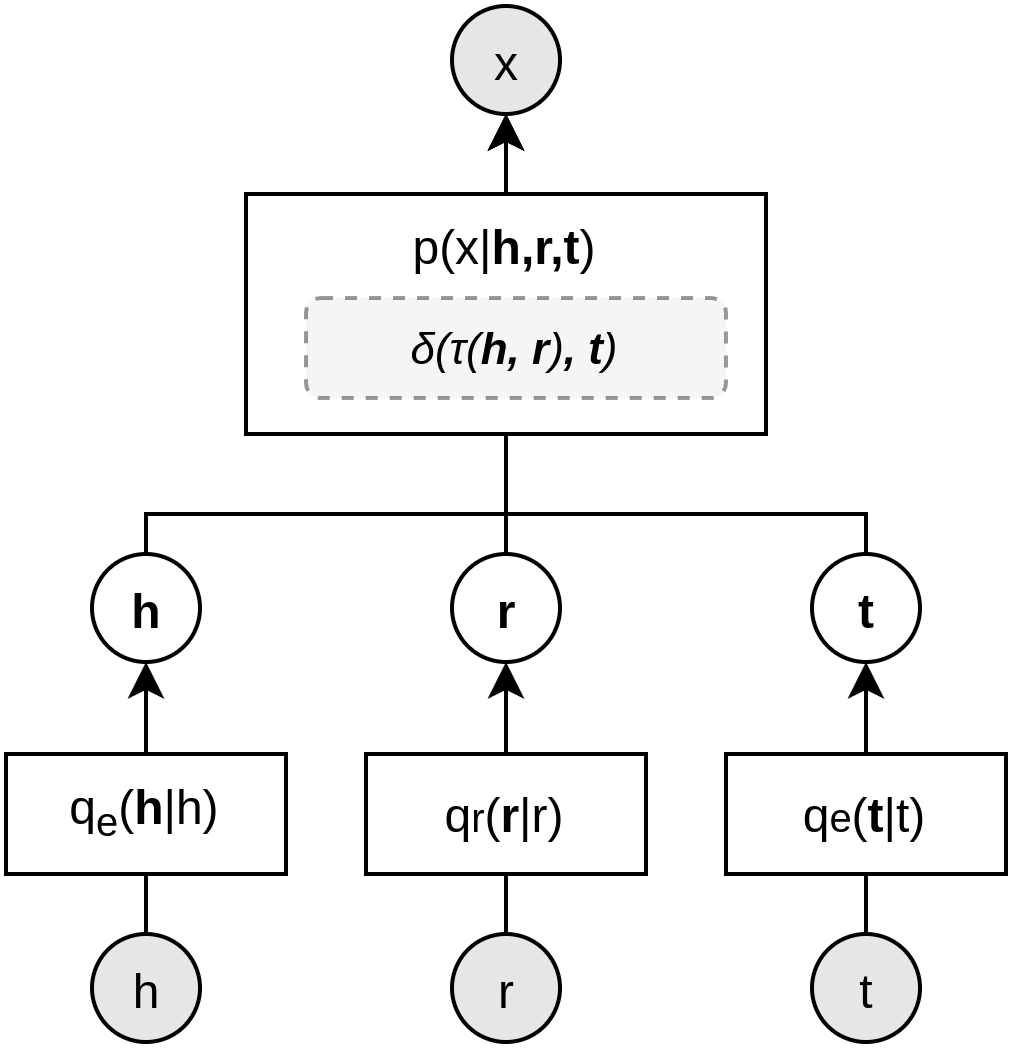
\includegraphics[width=1.\linewidth]{figures/base.png}
    \caption[Example of model diagram.]{Example of model diagram. The circles represent random variables, gray circles are observed, white circles unobserved. The boxes and arrows represent modeling decisions, for example here we model the probability of $x$ as being dependent on the embeddings $\vec{h}, \vec{r}, \vec{t}$. }
    %The gray rectangle containing $\sigma(\delta(\tau(\vec{h},\vec{r}),\vec{t}))$ gives specific information on the way that the distribution $p(x|\vec{h},\vec{r},\vec{t})$ is parameterized.}
    \label{fig:example_model_diagram}
\end{marginfigure}

This chapter describes and motivates the various ways in which we incorporate type information.
Some methods are original designs, for others we take inspiration from previous work.
The methods are described using both the notation introduced in the previous chapters, and using diagrams depicting the structure of the model (for example, a typical geometric model is depicted in Figure \ref{fig:example_model_diagram}).

\section{Objectives}\label{sec:method:objectives}%
The main objective is to answer the research question as given in Chapter \ref{ch:introduction}:
\begin{quote}
    \textit{(\textbf{RQ1})}
To what extent can type-information improve link-prediction performance? And,
\textit{(\textbf{RQ2})}
what method of incorporating the type-information is most effective?
\end{quote}
%
However, while answering our research question it might be useful to keep in mind some additional objectives. To maximize the utility of our investigations, we will keep in mind three secondary objectives, which are described below. Note that our methodology is not directly aimed at addressing these, but all things being equal, will try to nonetheless.

\subsection{Link Prediction as a proxy for general purpose embedding}
Knowledge Graph Embeddings may be used for a variety of downstream tasks such as: relation extraction, question answering, or recommender systems \mycitep{wang_knowledge_2017}. 
%Often the ability to predict links is still used as the primary objective during training. 
%This ability is regarded as indicative of
It will be useful to keep in mind how the different ways we incorporate type-information will affect these kinds of use cases.


\subsection{Anonymous entity embedding}
Using type information can allow us to embed entities that were not seen during training, as long as we know its type. 
%
To obtain such embeddings we need to model our embeddings as being conditioned on the types of the entity, i.e. $\vec{E}_i | C_{i,s}\!=\!c_{i,s}$.
Of particular interest is any model that accomplishes this without giving up the possibility of learning a specific embedding for the entities we do see during training.


% \subsection{Modeling uncertainty}
% Modeling the embeddings as probabilistic rather than point estimates (for example, like \mycite{he_learning_2015}) might be beneficial when it comes to incorporating type-information in the embeddings. For example, when learning embeddings for types using a point estimate to model a type, it seems we are at best learning a `prototypical' example of that type. With a distribution the variance can be tuned such that the probability mass covers all the space that the entities of that type exist in.


% An obvious way to improve upon KG2E is by using a type of normalizing flow such as Inverse Autoregressive Flow\cite{kingma_improved_2016}.

% One interesting avenue this method would open, is the ability to create a model where we first get $\vec{h}|h$, $\vec{r}|r$, $\vec{t}|t$ but then also have an additional posterior $\vec{h'},\vec{r'},\vec{t'}|\vec{h},\vec{r},\vec{t}$ such that the embeddings can be adapted by letting information flow between the different triple components. 
% %
% Of course you could just parameterize an approximate posterior $q(\vec{h'},\vec{r'},\vec{t'}|{h},{r},{t})$ from the beginning. But the downside of this is that we no longer have access to independent entity embeddings at all, only contextualized embeddings that are triple-specific.



\section{Using types to estimate prior probability of links}
\label{sec:method_type_linkprior}
%
The first method to be included in our experiments is the type-based prior introduced by \citeauthor{ma2017transt} in their paper on TransT (described in Section \ref{sec:transt}). 
It gives us an estimation of $p(h|r,t)$, $p(r|h,t)$, and $p(t|h,r)$.
It can easily be used in combination with any model to re-weight the scores assigned to each triple.
When used with a model that gives the likelihood of a triple, we can use the priors to get  approximated posteriors $p(h|r,t,x)$, $p(r|h,t,x)$, and $p(t|h,r,x)$.

By directly influencing the prediction for links, this approach is aimed at solving the primary objective. It does not address either of the additional objectives.

\paragraph{}\noindent
We do not include all configurations of TransT that \citeauthor{ma2017transt} propose. They distinguish between the configurations `type information', `multiple vectors' and `multiple+type'. In the first configuration the type-based prior is used to reweigh the scores as described above.
The second configurations refers to the representation of entities by multiple vectors. The number of vectors to be learned for each entity is based on the available type information (see Section \ref{sec:transt}). The last configuration combines the first two.
We include only the `type information' configuration, because any performance gain of the other configurations cannot easily be attributed to use of type-information, since it could also be attributed to the increase in the number of parameters.


\subsection{Type-linkprior only}
%
This method evaluates the type-based prior on its own.
We use only the score given by the prior to rank which triples are most likely to exist.
This gives us an indication of how informative the prior is, as well as a way to compare the datasets on the relative richness of their type information.
This configuration was not included in the experiments of \citeauthor{ma2017transt}.


\subsection{Type-linkprior+ScoringModel}
%
This method combines an existing ScoringModel, i.e. a model that already scores each triple, with the type-based prior. The final scores are those assigned by the ScoringModel multiplied by the estimated prior probability.
When the ScoringModel is TransE we obtain the configuration from which TransT derives its name.
This method is equivalent to \citeauthor{ma2017transt}'s `type information' configuration.


\section{Using types to construct the entity-embeddings}
%
Another way to use type information is to let each entity's set of types influence what the embedding of those entities will be. We experiment with three different kinds of embedders each with their own way of letting the types influence the entity-embeddings.
This type of model is displayed in Figure \ref{fig:type_for_entity_embeddings}.

\begin{marginfigure}
    \centering
    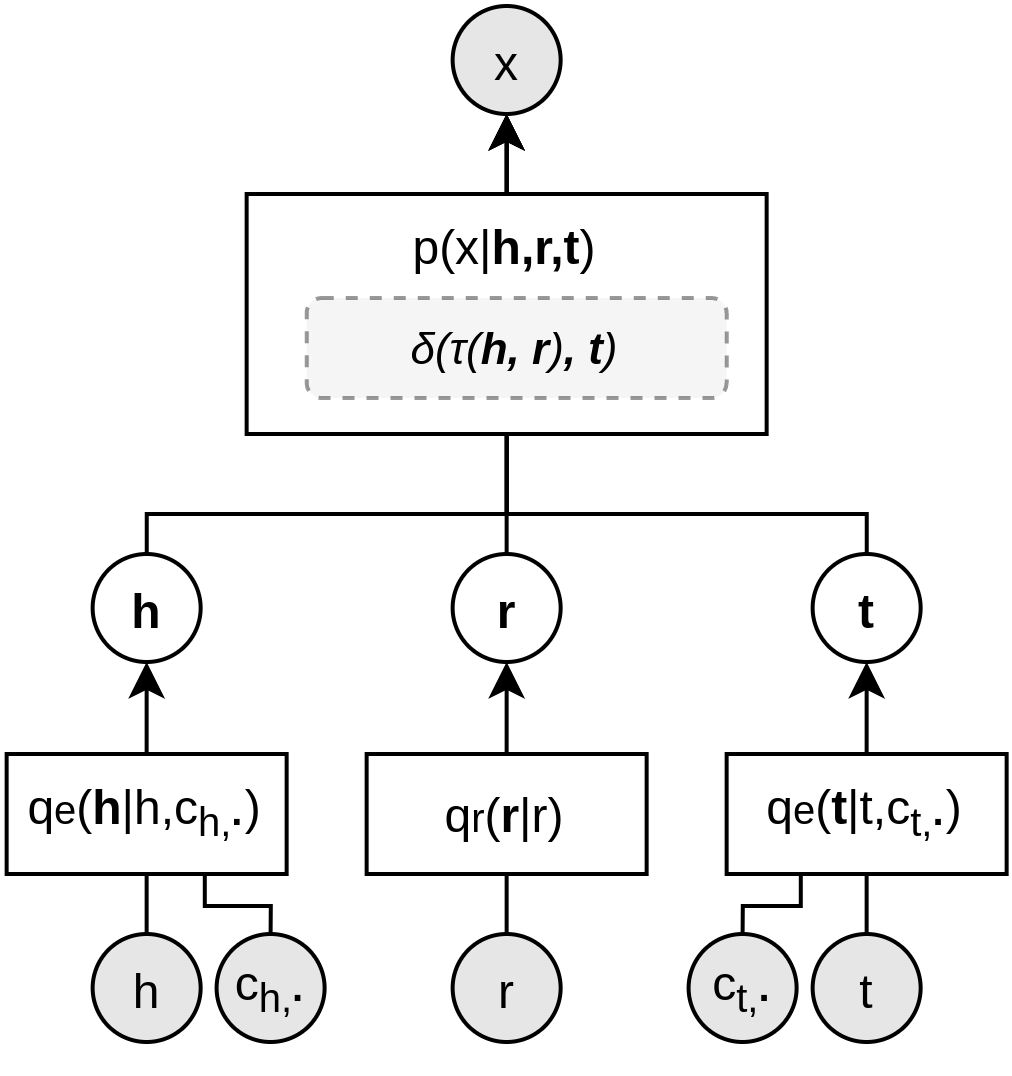
\includegraphics[width=\linewidth]{figures/type-embed.png}
    \caption[Model diagram with types for entity-embeddings.]{Diagram of model that utilizes types to construct entity-embeddings. }
    \label{fig:type_for_entity_embeddings}
\end{marginfigure}

% TYPE-MEAN
\subsection{Type-mean embedder}\label{sec:methods:type_mean}
This embedder is perhaps the simplest way of creating an entity's embedding from its types. Its main purpose is to serve as a baseline. 
%, showing what kind of performance is possible by including type-information in the entity-embeddings.
It learns embeddings for the types, and models an entity's embedding as the average of that entity's type embeddings, i.e.:
%\marginnote[2em]{We use $c_{i,\cdot}^+$ as short for $C_{i,\cdot} = True$.}
\begin{align}
    & \vec{C}_{s} | \theta_{s} && \simpnt \theta_{s} \\
%
%    & \vec{E}_i | C_{i,s} = c_{i,s} && = \underset{c_{i,s}}{\mathbb{E}} \left[ \vec{c}_s \right]
%    & \vec{E}_i | c_{i,1}^+, c_{i,2}^+, \dots, c_{i,Z}^+ && = \frac{1}{Z} \sum_{z=1}^{Z} \,\vec{c}_z
    & \vec{E}_i | c_{i,1}, c_{i,2}, \dots, c_{i,S} && 
    = \frac{\sum_{c_{i,z}} \vec{c}_z}{\sum_{c_{i,z}} 1} 
\end{align}
where $\theta_{s}$ are the model parameters that provide the point estimate for the $s$-th type's embedding.

\paragraph{Variant: adding entity offset embeddings.}
This variant learns an additional vector for each entity that we add to the mean of the type-vectors.
\begin{align}
    & \vec{E}_i | \epsilon_i, c_{i,1}, c_{i,2}, \dots, c_{i,S} && 
    = \frac{\sum_{c_{i,z}} \vec{c}_z}{\sum_{c_{i,z}} 1} + \epsilon_i
\end{align}
%
This addition could allow for more accurate embeddings for the entities, since two entities with the same types can now be specialized. 

This method could also be able to satisfy one of our secondary objectives. Specifically if the entity-offset is randomly dropped-out for some batches during training, it could allow us to embed both seen and unseen entities. Unseen entities are embedded by forgoing the entity-specific offset.
%
Furthermore the inclusion of the type-information in the entity-embeddings themselves may benefit downstream tasks.

% TYPE-ATTENTIVE
\subsection{Type-attentive embedder}
\begin{marginfigure}%[3.5cm]
    \centering
    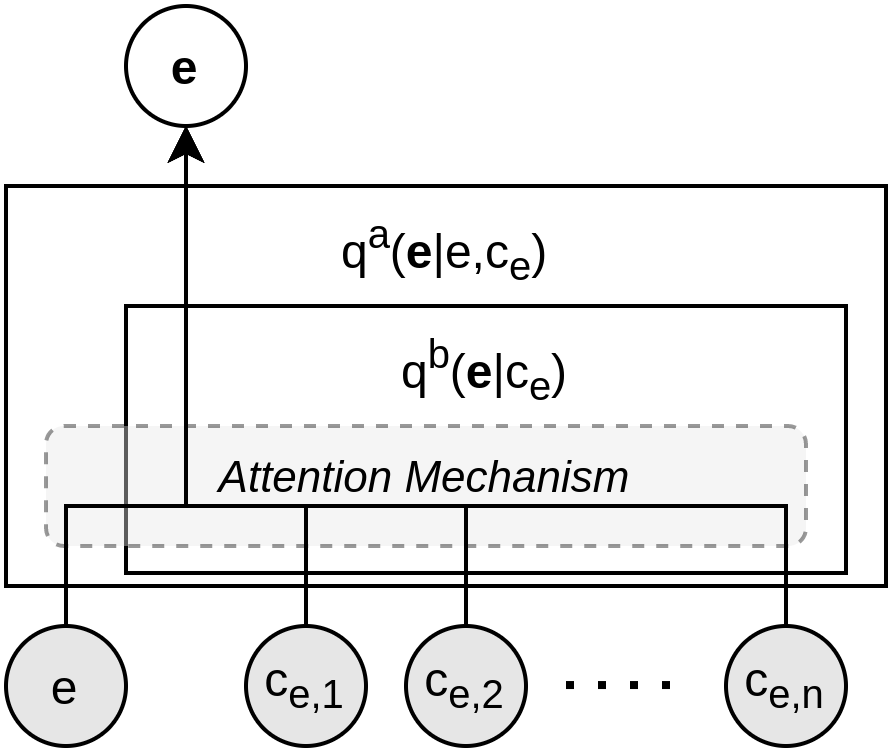
\includegraphics[width=\linewidth]{figures/type-attentive.png}
    \caption[Diagram of the type-attentive embedder.]{Diagram of the type-attentive embedder, depicting the two variants $q^a$ which includes the entity $e$ in the keys and values, and $q^b$ which does not. }
    \label{fig:type_attn_embed}
\end{marginfigure}

This embedder improves upon the type-mean embedder by learning to weight the type-embeddings differently for each entity. We do so with an attention mechanism:
\begin{align}
    & {q}_i             && =        ( \epsilon_i )^\top \\
    & {k}_i = {v}_i     && =        ( \theta_s | \mathcal{C}_{i,s})^\top \\
    & \vec{E}_i         && \simpnt  \mathrm{attn}(q_i, k_i, v_i)
\end{align}
where $\epsilon_i$ and $\theta_s$ are entity- and type-specific model parameters respectively.

\paragraph{Variant: adding the entity-vector to the keys and values.}
In this variant we allow the entity-vector to be included in the weighted average.
\begin{align}
    & {k}_i = {v}_i     && =        ( \epsilon_i ; \theta_s | c_{i,s})^\top 
\end{align}
This variant allows further specialization for each entity.

\paragraph{Mutual information loss.}
% hjelm_learning_2018
To encourage the inclusion of type information in the final entity-embeddings, we introduce an additional optimization objective. Taking inspiration from \mycite{hjelm_learning_2018}, we employ a mutual information based secondary objective.


%This idea is depicted in a diagram in Figure \ref{fig:type_attn_embed}. 

%\subsection{Idea}
%\begin{itemize}
    %\item Learn embeddings for entity-classes, as well as entities to get: $p(\vec{h}|c_h)$, $p(\vec{t}|c_t)$ and $p(\vec{h}|h)$, $p(\vec{t}|t)$. 
    %\item Combine those embeddings in an attention mechanism to also parameterize $p(\vec{h}|h,c_h)$ and $p(\vec{t}|t,c_t)$.
    %\item To meet requirement \ref{req:class-latent}, we would need to use $p(\vec{h}|c_h)$, $p(\vec{t}|c_t)$ to predict $x$ (some of the time) as an additional loss. 
    %\item Attention mechanism: 
    %    \begin{itemize}
    %        \item 1-N, keys = $\{ \vec{e} \}$, queries = values = $\{ \vec{e}, \vec{c}_{e,1}, %\dots, \vec{c}_{e,n} \}$ 
    %        \item $f_v(x) = x$; $f_q(x) = f_k(x) =  (x)$; \\ $out = \sum (f_k(x) \cdot f_q(x)) * %f_v(x)$
    %        \item if $\vec{e}$ is dropped (to train model on type alone) replace $f(\vec{e})$ %with $\vec{1}$.
    %    \end{itemize}
    %\item
%\end{itemize}


\section{Using types to provide additional supervision}
\subsection{Type-embedprior embedder}

The main intuition motivating this model is to think of types as distributions over entities. 
The most straightforward way to translate that intuition into a model, would be to sample from type-distributions to obtain our entity embeddings. 
However, each entity may have multiple types, and it is unclear how we could tractably sample from a set of type-distributions.

To avoid this difficulty, we therefore do not sample the entity embeddings from the type distributions, but instead learn independent entity embeddings that are nonetheless likely under their types' distributions.
\begin{align}
    & \vec{E}_i | \epsilon_i && \simpnt \epsilon_i \\
%
    & \vec{C}_{s} | \mu_s, \sigma_s && \sim N(\mu_s, \sigma_s)
\end{align}
To accomplish this, we introduce a second optimization objective. Besides the objective to maximize the likelihood of the data, we now also wish to maximize the likelihood of the entities under the distributions of their types, and minimize the likelihood of entities under the distributions of other types\sidenote{See \ref{sec:experiments:impl_type_embedprior} for more information on how we implement this.}:
\begin{align}
    \argmax_{\epsilon, \mu, \sigma} \quad 
    \prod_{C_{i,s}} f_{\vec{C}_{s}} ( \vec{e} ) 
  - \prod_{\lnot C_{i,s}} f_{\vec{C}_{s}} ( \vec{e} )
\end{align}
where $f_{\vec{C}_{s}}$ is the probability density function of $\vec{C}_{s}$.

\paragraph{Relation to other work.}
%\marginnote[2cm]{See Section \ref{} for how the type-embedprior may be extended to match \citeauthor{hao2019joie}'s method that includes a transformation before the distance is measured.}
\marginnote{\citeauthor{hao2019joie} also distinguish between two variants, one where the distance is calculated directly to the type vectors, and another where a transformation is applied to the type vectors first.
The variant with a transformation can also be reinterpreted probabilistically, if the transformation is implemented as a normalizing flow.} 
%After all a flow is nothing more than a transformation designed specifically to have a tractably calculable Jacobian determinant, which is what allows us to use it for a distribution.}
There exists an interesting parallel between the design of this embedder and the work of \citeauthor{hao2019joie} (described in Section \ref{sec:hao2019joie}).
We can think of our model as a probabilistic reinterpretation of the same ideas.
%
They too use a modified optimization objective, however their additional loss is not the likelihood of an entity under their types' distribution. Instead it is merely the distance between an entity embedding and its types' deterministic embeddings.
%
%

% \section{Type-prediction Loss}
% The goal here is to explicitly enforce the inclusion of type-information in our embeddings.
% This is inspired by \nameref{sec:semantically_smooth_knowledge_graph_embedding} which also organizes the embedding space by types, for which they observed increased performance.

\newpage
\section*{Overview}
%\todo[inline]{summarize, explain that we have now made clear which methods the `method' in the research question refers to}
%
Each of the methods we described use a strategy that we previously identified in the literature.
We can see an overview of the methods, the kinds of input information they have access to, and the strategies that they employ in Table \ref{tab:method_overview}.

%\begin{margintable}
\begin{table}
    \setlength{\tabcolsep}{5pt}
    \centering
    \begin{tabular}{lccr}
        \toprule
        \multirow{2}{*}{\textit{method}}     
                            & \multicolumn{2}{c}{\textit{inputs}} 
                                                        & \multirow{2}{*}{\textit{modification}} \\
        \cmidrule{2-3}
                            & $\epsilon_i$  & $c_{i,\mathbf{s}}$ \\
        \cmidrule{1-4}
        non-semantic        &\checkmark     &           & - \\
        \cmidrule{1-4}
        type-linkprior-only &               &\checkmark & triple score \\
        type-linkprior      &\checkmark     &\checkmark & triple score \\
        \cmidrule{1-4}
        type-mean           &               &\checkmark & \hspace{4em} entity-embeddings \\
        type-mean+          &\checkmark     &\checkmark & entity-embeddings \\
        type-attentive      &\checkmark     &\checkmark & entity-embeddings \\
        type-attentive-alt  &\checkmark     &\checkmark & entity-embeddings \\
        \cmidrule{1-4}
        type-embedprior     &\checkmark     &\checkmark & optimization objective \\
        \bottomrule
    \end{tabular}
    \caption[Overview of each method.]{Overview of each method, including the kinds of input (entity, type) each method has, as well as the strategy used to incorporate type-information.}
    \label{tab:method_overview}
\end{table}
%\end{margintable}
 
\chapter{Experiments}
\label{ch:experiments}
This chapter will describe what experiments have been performed to answer the research question formulated in Chapter \ref{ch:introduction}, and give the results of those experiments.
%
The description of the experiments includes implementation details of the methods described in the previous chapter, as well as the strategy employed for the hyper-parameter search.
%
The results are include both performance metrics resulting from the hyper-parameter searches, and  analyses of the methods aimed at confirming the methods are working as intended.

\section{Implementations}
We make the implementations of the methods described in Chapter \ref{ch:methodology} and the experiments described here freely available in the newly created SemKGE (Semantic KGE) repository,\sidenote[][0em]{\rurl{github.com/sfschouten/semantic-kge}} which was developed as a plugin to the LibKGE library\sidenote[][0em]{\rurl{github.com/uma-pi1/kge}}  \mycitep[0em]{broscheit_libkge_2020}.

\subsection{Type-linkprior}
% \todo[inline,caption={}]{
%     \begin{itemize}
%         \item explain learnable lambdas
%         \item 
%     \end{itemize}
% }
This method is implemented such that the variables $\lambda_{head}, \lambda_{relation}, \lambda_{tail}$ from Formulas \ref{formula:p_hrt}, \ref{formula:p_rht}, \ref{formula:p_thr} are learnable during training. As such, we introduce a hyper-parameter to control whether they are learned or not. If this hyper-parameter is set to true, the hyper-parameters that are normally used to set these values, now merely set their initial value.

%\subsection{Type-mean}
%

\subsection{Type-attentive}
The optimal learning rate for training a method like TransE can be quite high (\citeauthor{ruffinelli_you_2019} find an optimal learning rate of 0.25327).
Since the attention mechanism in the type-attentive embedder is the only part of the model that contains fully connected layers (which generally require lower learning rates), we tune the learning rate separately for that component. 


\subsection{Type-embedprior}\label{sec:experiments:impl_type_embedprior}
This method's additional optimization objective maximizes the difference in probability density assigned to an entity-embedding by that entity's types' distributions, and the density assigned by the other types' distributions.
We implement this by drawing one negative type sample for each type of each entity.


\subsection{Additional losses with constrained optimization.}
Optimizing with multiple objectives is often done by creating a weighted sum of loss terms.
But this strategy may be flawed, recently it was shown that this approach may fail even on small toy problems \mycitep{degrave_how_2021}. %mayne \sidenote on pareto front.
A potential solution is to construct a constrained optimization problem, where we identify one of our loss terms as the primary objective and incorporate the others as constraints. 
Using the Modified Differential Method of Multipliers \mycitep{platt_constrained_1987} allows us to utilize gradient descent with such a constrained optimization problem.
This method has been employed successfully with Variational Autoencoders \mycitep{rezende_taming_2018}, but should lead to more easily tunable hyperparameters regardless of the application.

As such the type-attentive's mutual information loss, and the type-embedprior's type-distribution density loss are both incorporated as constraints.


% \begin{align}
%     \argmax_{\epsilon, \mu, \sigma} \quad 
% &   p( x | \vec{h}, \vec{r}, \vec{t} ) \\[0.4em]
%     \text{subject to} \quad 
% &   u < \prod_{C_{h,s}} f_{\vec{C}_{s}} ( \vec{h} ) 
%       - \prod_{\lnot C_{h,s}} f_{\vec{C}_{s}} ( \vec{h} )\\
%     \text{and} \quad
% &   v < \prod_{C_{t,s}} f_{\vec{C}_{s}} ( \vec{t} )
%       - \prod_{\lnot C_{t,s}} f_{\vec{C}_{s}} ( \vec{t} ).
% \end{align}


\section{Datasets}
The datasets we use for our experiments are FB15K-237 \mycitep{toutanova_representing_2015}, WN18RR \mycitep{dettmers_convolutional_2018}, CoDEx-S and CoDEx-M \mycitep{safavi_codex_2020}.
%
The first two are well known benchmarks for Link Prediction \mycitep{ruffinelli_you_2019}.
They are the successors of the FB15K and WN18 datasets, which had been found to have test leakage \mycitep{rossi_knowledge_2021}.
The latter are two variants of a recently introduced set of benchmarks called CoDEx.  \citeauthor{safavi_codex_2020} show that CoDEx covers more diverse and interpretable content than FB15K-237, and that CoDEx is a more difficult . 
Statistics for each of these datasets can be seen in Table \ref{tab:dataset_statistics}.

%   \multirow{2}{*}{\fbox{\parbox[t][2.3em][s]{4.40em}{types\\per entity}}} &
%   \multirow{2}{*}{\fbox{\parbox[t][2.3em][s]{2.75em}{types\\in use}}} &
%   \multirow{2}{*}{\fbox{\parbox[t][2.3em][s]{2.50em}{total\\types}}} \\
\vspace{3cm}
\begin{table*}
\centering
    \begin{tabular}{@{}lrrrrrrrr@{}}
    \toprule
    \multirow{2}{*}{} &
      \multicolumn{1}{l}{\multirow{2}{*}{entities}} &
      \multicolumn{1}{l}{\multirow{2}{*}{relations}} &
      \multicolumn{3}{l}{triples} &
      \multirow{2}{*}{\parbox{4.70em}{\vspace{4pt}\setstretch{0.8}avg. types\\per entity}} &
      \multirow{2}{*}{\parbox{2.75em}{\vspace{1pt}\setstretch{0.8}types\\in use}} &
      \multirow{2}{*}{\parbox{2.50em}{\vspace{3pt}\setstretch{0.8}total\\types}} \\
    \cmidrule(lr){4-6}
     &
      \multicolumn{1}{l}{} &
      \multicolumn{1}{l}{} &
      \multicolumn{1}{l}{train} &
      \multicolumn{1}{l}{valid} &
      \multicolumn{1}{l}{test} &
       &
       \\ \midrule
    FB15K-237 & 14,541 & 237 & 272,115 & 17,535 & 20,466 & 12.422 & 3,865 & 4,054 \\
    WN18RR    & 40,943 &  11 &  86,835 &  3,034 &  3,134 &  1.000 &     4 &     4 \\
    CoDEx-S   &  2,034 &  42 &  32,888 &  1,827 &  1,828 &  1.619 &   502 & 3,443 \\
    CoDEx-M   & 17,050 &  51 & 185,584 & 10,310 & 10,311 &  1.253 & 1,505 & 3,443 \\ 
    \bottomrule
    \end{tabular}\vspace{1em}
\caption{Dataset statistics.}
\label{tab:dataset_statistics}
\end{table*}



\begin{figure*}
    \centering
    \begin{subfigure}[b]{0.32\textwidth}
        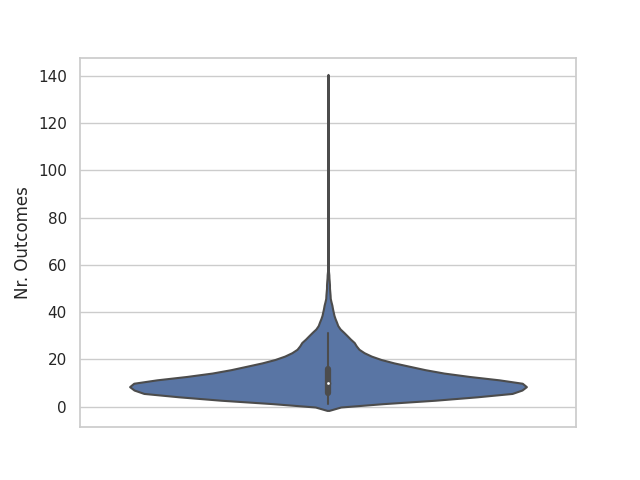
\includegraphics[trim=0cm 11mm 1cm 0pt, clip]{figures/datasets/fb15k-237.png}
        \caption{FB15K-237}
    \end{subfigure}
    \begin{subfigure}[b]{0.32\textwidth}
        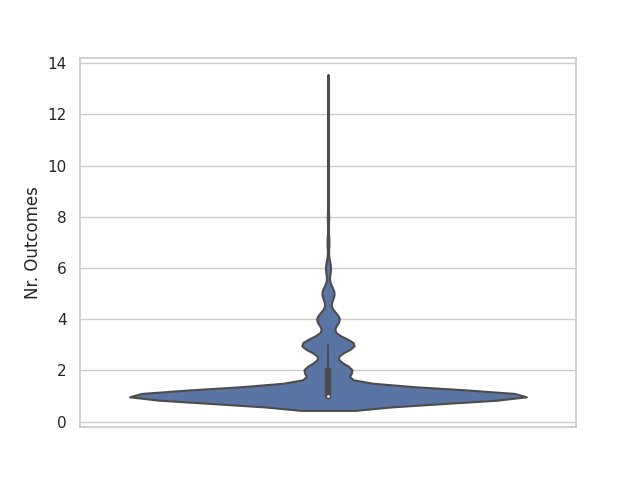
\includegraphics[trim=0cm 11mm 1cm 0pt, clip]{figures/datasets/codex-s.png}
        \caption{CoDEx-S}
    \end{subfigure}
    \begin{subfigure}[b]{0.32\textwidth}
        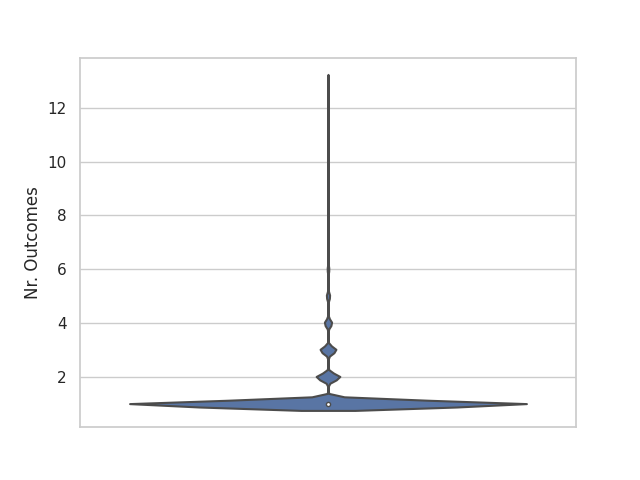
\includegraphics[trim=0cm 11mm 1cm 0pt, clip]{figures/datasets/codex-m.png}
        \caption{CoDEx-M}
    \end{subfigure}
    \caption[Distribution of number of types per entity.]{Distribution of number of types per entity across test portion of the datasets. The WN18RR dataset is omitted because it has exactly one type for each entity.}
    \label{fig:my_label}
\end{figure*}

%\FloatBarrier


\section{Technical Details}
All experiments were run on the SURFsara Lisa GPU cluster\sidenote[][2cm]{\rurl{userinfo.surfsara.nl/systems/lisa/description}}. 
The nodes we used had Nvidia GeForce 1080Ti GPUs with 11GB of VRAM.


\section{Evaluating \& Optimizing Link Prediction}
The Link Prediction task is evaluated as a ranking problem. Given a triple we know to be correct $(h, r, t)$ (those triples in the validation or test set), we use our model to predict what the head or tail should be, i.e. $(?, r, t)$ and $(h, r, ?)$. We rank all other entities on their likelihood of being the missing head or tail. 
The ranking that the model predicts is evaluated by what ranks are assigned to the original correct head and tail.

\paragraph{Evaluation metrics} used to quantify the quality of the rankings include: Mean Rank (MR), Mean Reciprocal Rank (MRR), and Hits@N.
The Mean Rank is the mean of the ranks assigned to the correct triples. This metric gives a number between one and the number of entities, the lower the better.
It is easily interpreted, but its sensitivity to outliers is causing it to be abandoned in favor of MRR \mycitep[]{rossi_knowledge_2021}.
The Mean Reciprocal Rank is the mean of multiplicative inverse of the ranks. It gives a number between 0 and 1, the higher the better. It is much less sensitive to outliers.
Hits@N gives the percentage of correct triples with an assigned rank below N, the higher the better.

These metrics can be calculated in two different ways, they can be computed \textit{raw} or \textit{filtered}. This choice determines how we treat other predictions of heads/tails that also correct triples, that are not the triple for which we are currently doing head/tail prediction. If we report the \textit{raw} metrics, we leave these other correct triples alone, if we report the \textit{filtered} metrics we filter them out. The \textit{filtered} metrics are generally preferred because we do not care about the model ranking other correct triples above the currently evaluated triple.

\paragraph{Loss functions} used to optimize for these ranking metrics need special attention, because the metrics themselves are not continuous. This is because these metrics require sorting the scores assigned to triples in order to compute their rank. So to optimize with gradient descent, we use separate loss functions as a proxy for these metrics. 

One possibility is to model the truth of a triple as being sampled from a Bernoulli distribution.  
\begin{align}
    & X | \vec{h}, \vec{r}, \vec{t}
&& \sim \text{Bernoulli}( \sigma( score( \vec{h}, \vec{r}, \vec{t} ) ) )
\end{align}
Where $\sigma$ is a function that maps the scores to $(0,1)$.
The difference between the model distribution and the data distribution is then quantified as the Binary Cross Entropy (BCE) loss.

Alternatively we can think of the true triples as being sampled from a set of triples $\mathcal{S}_{(h,r,t)}$.
\begin{align}
    & p(\bm{\mathcal{S}}_{(h,r,t)})  && = \sigma \left(  score(\vec{h'}, \vec{r'}, \vec{t'}) \,|\, (\vec{h'}, \vec{r'}, \vec{t'}) \in \bm{\mathcal{S}}_{(h,r,t)} \right)^\top
\\
    & K^+ | \bm{\mathcal{S}}_{(h,r,t)} && \sim \text{Categorical}(|\bm{\mathcal{S}}_{(h,r,t)}|, p(\bm{\mathcal{S}}_{(h,r,t)}))
\\
    & X^{(k')} && = [k' = k^+]
\end{align}
Where $\sigma$ is the softmax function, $S_{(h,r,t)}$ is the set of triples and $\vec{S}_{(h,r,t)}$ are their embeddings. In practice this set is based on a triple $(h,r,t) \in \mathcal{D}^+$, it includes that triple itself and a set of negative triples constructed from the original.
When modeled this way the difference between the model and data distribution is quantified as the Categorical Cross Entropy loss.

Other loss functions like Margin Ranking and Squared error are sometimes also used. However, in contrast to the losses mentioned above, these others are optimal for none of the methods included in the hyper-parameter search performed by \citeauthor{ruffinelli_you_2019}.

\paragraph{Training approaches} differ from each other by how batches of triples are constructed. Negative sampling is an approach that first samples triples from the training data, and then constructs set of negatives for each triple by corrupting one of the triple's components. \citeauthor{ruffinelli_you_2019} implement two other approaches, 1vsAll, and KvsAll. The 1vsAll approach is similar to negative sampling but adds every possible way of corrupting a triple as a negative, even if the resulting triples occur in the training data. 
The KvsAll approach only corrupts either the head or tail, and contrary to 1vsAll, labels all that occur in the training data as positive, and only those that do not as negative.

\section{Hyper-parameter Searches}
Our main experiment is an extensive hyper-parameter search. 
For each of the methods described in Chapter \ref{ch:methodology}, we use TransE as the underlying KGE model.
%
The strategy employed for the hyper-parameter searches is based on the strategy used in \mycite[4em]{ruffinelli_you_2019}. Each search is based on 30 rounds of parameters drawn from a Sobol sequence \mycitep[]{sobol1967distribution}. \citeauthor{ruffinelli_you_2019} follow this with 15 rounds of Bayesian optimization, but since they report that this has minimal effect we do not include these rounds. %\todo{decide definitively}


\subsection{Training}
We use a Categorical Cross Entropy loss, minimizing the KL Divergence between the model and data distributions, and use negative sampling as our training strategy. These two decisions were shown by \citeauthor{ruffinelli_you_2019} to be optimal for the TransE KGE model. 

We use a `shared' implementation of negative-sampling, meaning that the same negative samples are used for each triple in a batch. Note that it is ensured that a triple does not get itself as a negative.

\paragraph{}\noindent%
An extensive overview of which hyper-parameters were tuned can be found in Appendix \ref{apx:hyperparameter_search}

\begin{table}[p]
    \def\fn{\hspace{2pt}} % footnote columns
    \setlength{\tabcolsep}{5pt}
    \centering
    \begin{tabular}{lr@{\fn}lr@{\fn}lr@{\fn}lr@{\fn}l}
        \toprule
        \textit{name}
        &\multicolumn{2}{l}{WN18RR}
                    &\multicolumn{2}{l}{FB15K-237}   
                           & \multicolumn{2}{l}{CoDEx-S}   
                                        & \multicolumn{2}{l}{CoDEx-M} \\
        \cmidrule{1-9}
        non-semantic        & 0.226 && 0.308    && 0.354    && 0.306   \\
        \cmidrule{1-9}
        type-linkprior-only & 0.000 && 0.140    && 0.094    && 0.051   \\
        type-linkprior      & 0.191 && 0.324    && 0.354    && 0.284   \\
        \cmidrule{1-9}
        type-mean           & 0.723 && 0.272    && 0.446    && 0.357   \\
        type-mean+          & 0.174 && 0.319    && 0.350    && 0.274   \\
        type-attentive      & -     &&\textbf{0.615}&%\footnotemark
                                                 &\textbf{0.612}
                                                            &&\textbf{0.477}   \\
        type-attentive-alt  &\textbf{0.816}
                                    && 0.298    && 0.341    && 0.456   \\
        \cmidrule{1-9}
        type-embedprior     & 0.243 && 0.316    && 0.378    && 0.298   \\
        \bottomrule
    \end{tabular} \vspace{1em}
    \caption[MRR obtained by each method for best set of hyperparameters.]{Mean Reciprocal Rank obtained by each method for best set of hyperparameters. } \label{tab:hyperparam-search-results1}
\end{table}
%\addtocounter{footnote}{-1}
%\marginnote{\textsuperscript{\thefootnote\ }test}
%\todo{} 
%\addtocounter{footnote}{1}
%\marginnote{\textsuperscript{\thefootnote\ }test}


\begin{table}[p]
    \def\fn{\hspace{2pt}} % footnote columns
    \setlength{\tabcolsep}{5pt}
    \centering
    \begin{tabular}{lr@{\fn}lr@{\fn}lr@{\fn}lr@{\fn}l}
        \toprule
        \textit{name}
                &\multicolumn{2}{c}{WN18RR}
                            &\multicolumn{2}{c}{FB15K-237}   
                                           & \multicolumn{2}{c}{CoDEx-S}   
                                                                & \multicolumn{2}{c}{CoDEx-M} \\
        \cmidrule{1-9}
        non-semantic         & 1774.06     && 176.93       && \textbf{43.78}            && \textbf{289.89}   \\
        \cmidrule{1-9}
        type-linkprior-only  & 19581.08    && 686.44	   && 290.47           && 4655.25  \\
        type-linkprior       & 4617.39   && \textbf{158.69}       && 49.45     && 434.35   \\
        \cmidrule{1-9}
        type-mean            & 9714.45     && 233.67       && 88.20            && 1959.57  \\
        type-mean+           & 5912.00     && 171.31       && 54.84            && 582.91   \\
        type-attentive       & -           && 5374.72        &%\footnotemark
                                                           & 78.17             && 984.77   \\
        type-attentive-alt   & \textbf{1557.96}     && 188.45       && 54.46            && 967.30   \\
        \cmidrule{1-9}
        type-embedprior      & 3185.04     && 171.81       && 46.87            && 571.06   \\
        \bottomrule
    \end{tabular} \vspace{1em}
    \caption[MR obtained by each method for best set of hyperparameters.]{Mean Rank obtained by each method for set of hyperparameters with highest MRR.} \label{tab:hyperparam-search-results2}
\end{table}
%\addtocounter{footnote}{-1}
%\marginnote{\textsuperscript{\thefootnote\ }test}
%\addtocounter{footnote}{1}
%\marginnote{\textsuperscript{\thefootnote\ }test}

\begin{table}[p]
    \def\fn{\hspace{2pt}} % footnote columns
    \setlength{\tabcolsep}{5pt}
    \centering
    \begin{tabular}{lr@{\fn}lr@{\fn}lr@{\fn}lr@{\fn}l}
        \toprule
        \textit{name}
                &\multicolumn{2}{c}{WN18RR}
                            &\multicolumn{2}{c}{FB15K-237}   
                                           & \multicolumn{2}{c}{CoDEx-S}   
                                                                & \multicolumn{2}{c}{CoDEx-M} \\
        \cmidrule{1-9}
        non-semantic         & 51.53    && 49.90    && 64.37    && 46.65  \\
        \cmidrule{1-9}
        type-linkprior-only  & 00.00    && 21.91	&& 18.56    && 7.85   \\
        type-linkprior       & 43.75	&& 51.14    && 58.73    && 44.68    \\
        \cmidrule{1-9}
        type-mean            & 72.33    && 40.89    && 64.50    && 47.21  \\
        type-mean+           & 42.55    && 49.02    && 57.85    && 42.22  \\
        type-attentive       & -        && \textbf{61.57}     &%\footnotemark
                                                    & \textbf{83.03}     && \textbf{54.09}  \\
        type-attentive-alt   & \textbf{82.23}    && 47.05    && 58.35    && 51.85  \\
        \cmidrule{1-9}
        type-embedprior      & 63.25    && 49.57    && 62.62    && 45.05  \\
        \bottomrule
    \end{tabular} \vspace{1em}
    \caption[Hits@10 obtained by each method for best set of hyperparameters.]{Hits@10 (\%) obtained by each method for best set of hyperparameters. }\label{tab:hyperparam-search-results3}
\end{table}
%\addtocounter{footnote}{-1}
%\marginnote{\textsuperscript{\thefootnote\ }test}
%\addtocounter{footnote}{1}
%\marginnote{\textsuperscript{\thefootnote\ }test}

\subsection{Results}\label{sec:experiments:results}
The results of this hyper-parameter search can be seen in Tables \ref{tab:hyperparam-search-results1} (MRR), \ref{tab:hyperparam-search-results2} (MR), and \ref{tab:hyperparam-search-results3} (Hits@10).

No search was done for the type-attentive embedder on the WN18RR dataset. Using the type-attentive embedder on that dataset is not productive given that the dataset has exactly one type per entity. 
We do include the type-attentive-alt method since its attention mechanism can still learn to weigh the type representation against the entity representation.
%The type-mean embedder can always achieve the same performance with less parameters. 

%\todo[inline]{include runtimes in some capacity}

\section{Analysis}
Among the results are observations both expected and unexpected.
As expected, we see a clear correlation between the performance of the type-linkprior-only model and the type-linkprior model.
Overall we see a modest improvement over the non-semantic baseline.

However, among the type-mean and type-attentive models we see unexpected high performance for the simplest type-mean model. We also see the variants which allow entity-specific specialization underperform their counterparts. Both of these observations will require further analysis to understand.

The type-embedprior method induces a modest improvement in MRR for all but the CoDEx-M dataset.





\subsection{Type-linkprior[-only]: hyper-parameters}

In Table \ref{tab:linkprior-only-hparams} we can see the hyper-parameters for the type-linkprior-only method and the values that obtained the highest MRR for each dataset. 
Because this method fails to obtain a positive MRR or Hits@10 for the WN18RR dataset, the hyper-parameter values found for that dataset do not reflect anything meaningful.
For the other datasets we can see that the values found for the hyperparameters are similar.
Furthermore, we can see that optimizing the $\lambda$ parameters using gradient descent was not useful.

\todo{check if hyperparameters found for Type-linkprior are roughly same as only}

\begin{table}[ht]
    \def\fn{\hspace{2pt}} % footnote columns
    \setlength{\tabcolsep}{5pt}
    \centering
    \begin{tabular}{lr@{\fn}lr@{\fn}lr@{\fn}lr@{\fn}l}
        \toprule
                &\multicolumn{2}{c}{WN18RR}
                            &\multicolumn{2}{c}{FB15K-237}   
                                           & \multicolumn{2}{c}{CoDEx-S}   
                                                                & \multicolumn{2}{c}{CoDEx-M} \\
        \cmidrule{1-9}
        $\rho$                  & 0.455 && 0.179 && 0.079 && 0.172 \\
        \cmidrule{1-9}
        $\lambda_{head}$        & 0.548 && 0.877 && 0.919 && 0.862 \\
        $\lambda_{relation}$    & 0.780 && 0.026 && 0.122 && 0.095 \\
        $\lambda_{tail}$        & 0.746 && 0.805 && 0.714 && 0.717 \\
        \cmidrule{1-9}
        learn\_lambda           & true  && false && false && false \\
        \bottomrule
    \end{tabular} %\vspace{1em}
    \caption{The hyperparameters specific to the type-linkprior-only that were used to obtain the highest MRR.} 
    \label{tab:linkprior-only-hparams}
\end{table}


\subsection{Type-mean: performance}\label{sec:analysis:type_mean_performance}
The type-mean method outperforms the non-semantic baseline for three out of four datasets. 
This is surprising as this is the simplest method we test. By only learning separate vectors for each type, rather than each entity, it uses less parameters than the non-semantic baseline. 
The performance is most striking for the WN18RR dataset, where it gets an MRR score of $0.7233$\,. 
Since this dataset has only 4 types, and 11 relations, the number of vectors it uses to obtain this score is only 15 (!).
The entity's representation is calculated by averaging the representations of that entities types. Because WN18RR has only one type for each entity, we are effectively substituting each entity with its type. 

To understand why this results in high predictive performance, we can take a deeper look at the statistics of the WN18RR dataset. In particular we look at each relation's type-statistics, i.e. how many links exist between each type for that relation. These statistics are displayed in Table \ref{tab:wn18rr-relation1-type-statistics}.
%
\begin{table}
    \centering
    \begin{tabular}{lrrrr}
        \toprule
                    & \textit{NN} & \textit{VB} & \textit{JJ} & \textit{RB}  \\
        \cmidrule{1-5}
        \textit{NN} & 27826 (79.97\%) & 38 (00.11\%)   & 11 (00.03\%) & 4 (00.01\%)  \\ %noun
        \textit{VB} & 78 (00.22\%)    & 6791 (19.52\%) & 9 (00.03\%)  & 11 (00.03\%) \\ %verb
        \textit{JJ} & 11 (00.03\%)    & 7 (00.02\%)    & 0 (00.00\%)  & 0 (00.00\%)  \\ %adjective
        \textit{RB} & 7 (00.02\%)     & 3 (00.01\%)    & 0 (00.00\%)  & 0 (00.00\%)  \\ %adverb
        \bottomrule
    \end{tabular}
    \label{tab:wn18rr-relation1-type-statistics}
    \caption{Type statistics for most frequently occurring relation in WN18RR.}
\end{table}
%
In this table we can see that almost all of this relation's links are between a noun (NN) and another noun, or between a verb (VB) and another verb. This means that using only this information we can rank all potential links between two nouns first, and rank links between two verbs after that.
The other relations in the dataset have similar statistics, with one or two combinations of types being far more frequent than the rest. \todo{OPTIONAL: add in appendix}

Evidently for WN18RR statistics such as those found in Table \ref{tab:wn18rr-relation1-type-statistics} are informative enough to obtain very high performance on the Link Prediction task. However this does come at a cost, we now only have an embedding for each type, not each entity. If Link Prediction is the only concern then this might be a good tradeoff, but if the goal was to have a general-purpose knowledge graph embedding, it likely is not.

This method seems to also do very well for the CoDEx datasets, although not as well as for WN18RR. Type-mean does not perform well for FB15K-237. This is unsurprising when we look at the number of types per entity for each dataset. An average 1.62 and 1.25 types per entity for the CoDEx-S and CoDEx-M datasets puts them only just above the 1.0 of WN18RR. But FB15K-237 has an average of 12.42 types per entity (see Table \ref{tab:dataset_statistics}). With CoDEx most entities still have one type, like on WN18RR, but with FB15K-237 this is not the case. And without (mostly) a single type per entity the type-statistics cannot be represented like is possible for WN18RR.

Type-mean+'s performance is much more similar to the non-semantic baseline.
We see a modest improvement in MRR for FB15K-237 and about equal MRR for the CoDEx-S dataset.
For the WN18RR and CoDEx-M datasets this method show a decrease in MRR. 
It seems that this method's additional entity-specific representation creates an inductive bias that keeps it from learning the same behavior we see for the type-mean method.


\subsection{Type-attentive: attention weight distributions}
\label{sec:experiments:type_attentive}
\begin{figure*}
    \centering
    \caption[Scatter plot of metric entropy for CoDEx-S.]{Scatter plot of metric entropy over the number of outcomes for the CoDEx-S dataset.}
    \begin{subfigure}[b]{0.486\columnwidth}
        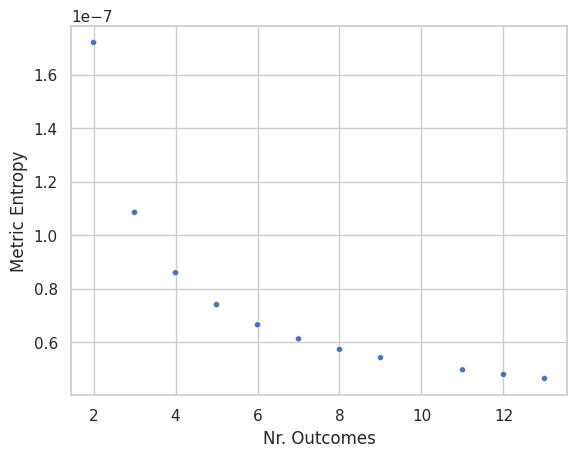
\includegraphics{figures/analysis/codex-s_scatter_nr_types_vs_metric_entropy.png}
        \caption{Type-attentive}
    \end{subfigure}
    \begin{subfigure}[b]{0.489\columnwidth}
        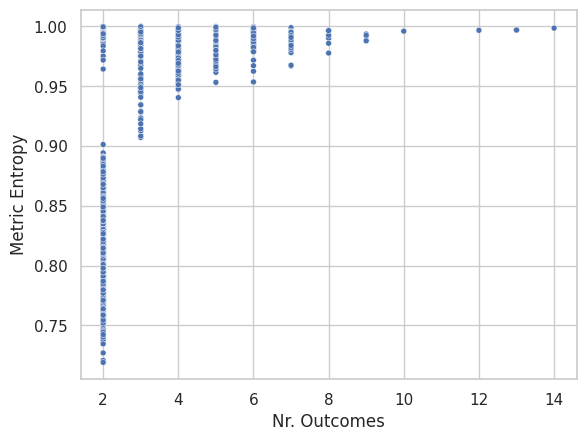
\includegraphics{figures/analysis/codex-s_alt_scatter_nr_types_vs_metric_entropy.png}
        \caption{Type-attentive-alt}
    \end{subfigure}
    \label{fig:metric_entropy_vs_nr_types_attentive_codex_s}
\end{figure*}

The intuition behind the type-attentive method was to have a weighted average between type representations rather than a simple mean. Like the type-mean method we see unexpectedly high MRR for the type-attentive method. We see even higher performance for this method, now for FB15K-237 too. In all likelihood because of similar reasons as the type-mean's high performance. This method can do even better at representing the type-statistics by learning to pick the one type that is most representative of each entity using the attention mechanism. To confirm this is the case we look at the attention weights as a probability distribution, and measure its Shannon Entropy to determine if most attention is paid to one or a few types or if the attention is fairly spread out.


%
In Figure \ref{fig:metric_entropy_vs_nr_types_attentive_codex_s} we can see a scatter plot of the Metric Entropy\sidenote[][2.2cm]{Metric Entropy is a normalized variant of the regular Shannon Entropy. It is obtained by dividing the Shannon Entropy by the information length (in bits, i.e. $log_2(|X|)$ where $|X|$ is the number of possible outcomes of the random variable). } of the attention weights for the type-attentive and type-attentive-alt methods when applied to the CoDEx-S dataset. We can see that the type-attentive method is assigning very low entropy weights to the type-vectors, regardless of the number of types of the entity\sidenote[][]{Note that for the type-attentive method the number of outcomes is often one (because that entity has only one type). These cases are not displayed in the plot, as Metric Entropy is undefined in those cases.}. This confirms that the the type-attentive method is choosing one type for each entity, using the type-statistics only to achieve high predictive performance.
%
The entropy for the type-attentive-alt variant looks rather different, its attention distributions are relatively high entropy.
This time the method seems to operate more like intended, taking in information from a variety of its types. Unfortunately, with an MRR that is slightly below the non-semantic baseline, this does not result in an increase in performance.

%
\begin{figure*}[t]
    \vspace{0.5cm}
    \centering
    \caption[Scatter plot of metric entropy for CoDEx-M.]{Scatter plot of metric entropy over the number of outcomes for the CoDEx-M dataset.}
    \begin{subfigure}[b]{0.50\columnwidth}
        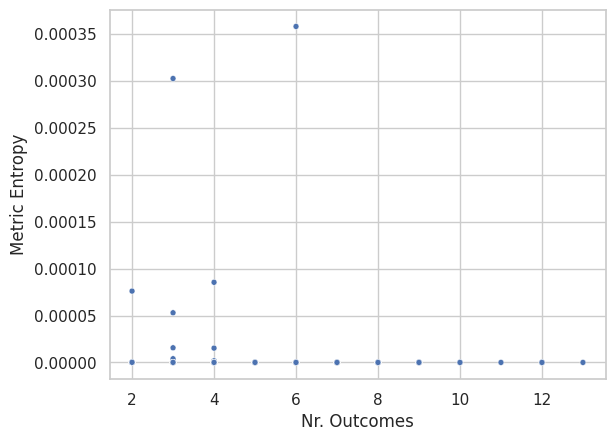
\includegraphics{figures/analysis/codex-m_scatter_nr_types_vs_metric_entropy.png}
        \caption{Type-attentive}
    \end{subfigure}
    \begin{subfigure}[b]{0.492\columnwidth}
        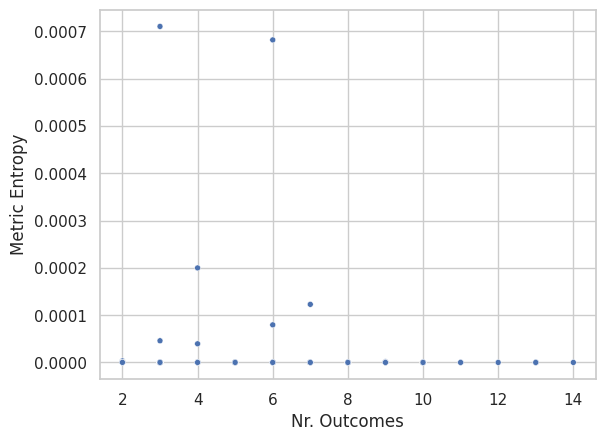
\includegraphics{figures/analysis/codex-m_alt_scatter_nr_types_vs_metric_entropy.png}
        \caption{Type-attentive-alt}
    \end{subfigure}\vspace{-1em}
    \label{fig:metric_entropy_vs_nr_types_attentive_codex_m}
\end{figure*}
%
In Figure \ref{fig:metric_entropy_vs_nr_types_attentive_codex_m} we can see the same type of plot but for the CoDEx-M dataset. Here we see that entropy is low for both of the method's variants, which explains why performance for both is similar. It seems that in rare cases even the type-attentive-alt method can uncover this type-statistics only mode where it attends only to a single representative type.


% \todo[inline,caption={}]{
%     \begin{itemize}
%         \item type attentive most attended as label for the types in TSNE
%     \end{itemize}
% }

\begin{table}%
    \def\fn{\hspace{2pt}} % footnote columns
    \setlength{\tabcolsep}{5pt}%
    \centering%
    \begin{tabular}{lr@{\fn}lr@{\fn}lr@{\fn}l}%
        \toprule%
                        &\multicolumn{2}{c}{FB15K-237}   %
                                           & \multicolumn{2}{c}{CoDEx-S}   %
                                                                & \multicolumn{2}{c}{CoDEx-M} \\
        \cmidrule{1-7}
        lr (default)    & $3.6 \cdot 10^{-2}$ && $1.7 \cdot 10^{-4}$ && $3.6 \cdot 10^{-2}$ \\
        lr (attn)       & $3.9 \cdot 10^{-1}$ && $6.6 \cdot 10^{-1}$ && $3.9 \cdot 10^{-1}$ \\
        \bottomrule
    \end{tabular} %\vspace{1em}
    \caption{Type-attentive learning rates for runs with best MRR.} %
    \label{tab:type-attn-lr}%
\end{table}%
%
\subsection{Type-attentive: hyper-parameters}\label{sec:analysis:type_attn_hparams}
In Table \ref{tab:type-attn-lr} we can see that the attention mechanism's learning rate is tuned to a higher value than we see for the rest of the model. 
The original intent of the separately tuned learning rate was to allow the attention mechanism to use a lower learning rate, not higher. It is possible that these learning rates play a role in reaching the low entropy modes.
%
The mutual information hyper-parameter was set below zero (disabled) for each dataset.

\subsection{Type-embedprior: learned distributions} \label{sec:analysis:type_embed_dist}
The intuition behind this method is that entities of the same type are similar, and should therefore be close to each other in the embedding space. Specifically, we construct distributions for each type and want the embedding of entities of those types to be likely under those distributions, and only those distributions.
To measure how well the learned distributions match this intuition, we now look at the degree of overlap between distributions. We hope that the distributions of types that do not have any entities in common also do not overlap in the embedding space.
We quantify the extent to which types have entities in common with the Jaccard Index, and  the degree of overlap with the Bhattacharyya Coefficient.

\begin{figure}
    \centering                             % left bottom right top
    \includegraphics[width=1.05\textwidth, trim=2mm 2mm 4mm 4mm, clip]
    {figures/analysis/embedprior/fb15k-237_scatter_typepair_jaccard_vs_bhattacharyya.png}
    \caption[Plot depicting Jaccard index of type pairs with the Bhattacharyya Distance between the learned distributions of those pairs.]{Combination of scatter plot, univariate KDE curves, and a linear regression fit, depicting the relation between the Jaccard Index of type pairs (as measured when considering types as sets of entities), and the Bhattacharyya Coefficient between the learned type distributions of said type pairs.}
    \label{fig:embedprior_jaccard_vs_bhattacharyya}
\end{figure}
A scatter plot of type-pairs with these two quantities on the x- and y-axis respectively can be seen in Figure \ref{fig:embedprior_jaccard_vs_bhattacharyya}. This figure also shows a linear regression fit, and displays the cardinality of the union of the two type sets using the color of the points, where bright yellow are the lowest and dark blue the highest cardinality\sidenote[][]{To reduce the total number of points and improve the utility of the plot, type-pairs with a Jaccard Index below 0.1 were left out. As were type-pairs with fewer than 10 entities between them, and types paired with themselves.}.
We see a clear correlation between the two quantities, but also see that it is mostly one-way. In an ideal scenario the points in the plot would form a diagonal line, showing perfect correlation. Instead, we observe that most points occur above this hypothetical line. This indicates that types with a lot of entities in common also overlap in the embedding space, but types that do not have many entities in common, may still overlap considerably in the embedding space. We also observe that the type-pairs with the most entities between them exhibit more overlap in the embedding space, which is to be expected.


\subsection{Type-embedprior: hyper-parameters}\label{sec:analysis:type_embed:hparam}
The type-embedprior embedder seeks to make the entity-embeddings likely under their type-distributions. To do this it uses a minimum constraint on log-density assigned by the correct types minus the log-density assigned by other types. In other words, an entity's true types must assign at least some number of times more density to the entity's embedding, than other types do.
\begin{table}
    \def\fn{\hspace{2pt}} % footnote columns
    \setlength{\tabcolsep}{5pt}
    \centering
    \begin{tabular}{lr@{\fn}lr@{\fn}lr@{\fn}lr@{\fn}l}
        \toprule
                &\multicolumn{2}{c}{WN18RR}
                            &\multicolumn{2}{c}{FB15K-237}   
                                           & \multicolumn{2}{c}{CoDEx-S}   
                                                                & \multicolumn{2}{c}{CoDEx-M} \\
        \cmidrule{1-9}
        min log-density $\Delta$ & 6.982 && 7.470 && 7.470 && 6.588 \\
        \bottomrule
    \end{tabular} %\vspace{1em}
    \caption[Differences in log-density required of entity-embedding under type distributions.]{Minimum difference in log-density required of entity-embedding under the distributions of that entities types and set of sampled negative types (for the best performing model from the hyper-parameter search).} \label{tab:min_log_density_delta}
\end{table}

In Table \ref{tab:min_log_density_delta} we can see the value of the hyper-parameter that governs the minimum difference in log-density required, for the best run from the hyper-parameter search.
We can see that for each dataset a similar value is selected. 
\begin{figure*}
    \centering
    \begin{subfigure}[b]{0.50\columnwidth}
        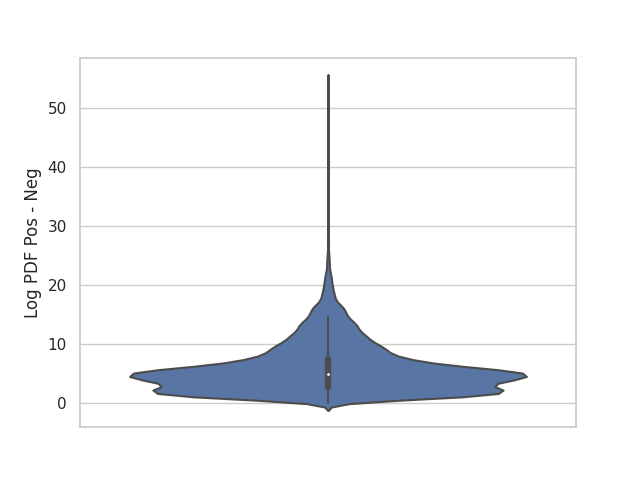
\includegraphics[trim=0cm 11mm 1cm 0pt, clip]{figures/analysis/embedprior/fb15k237_analysis_prior_lpdf_diff.png}
        \caption{FB15K-237}
    \end{subfigure}
    \begin{subfigure}[b]{0.492\columnwidth}
        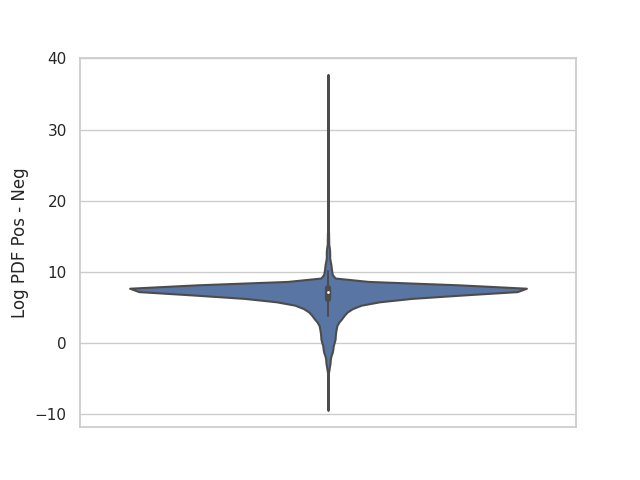
\includegraphics[trim=0cm 11mm 1cm 0pt, clip]{figures/analysis/embedprior/wnrr_analysis_prior_lpdf_diff.png}
        \caption{WN18RR}
    \end{subfigure}
    \begin{subfigure}[b]{0.492\columnwidth}
        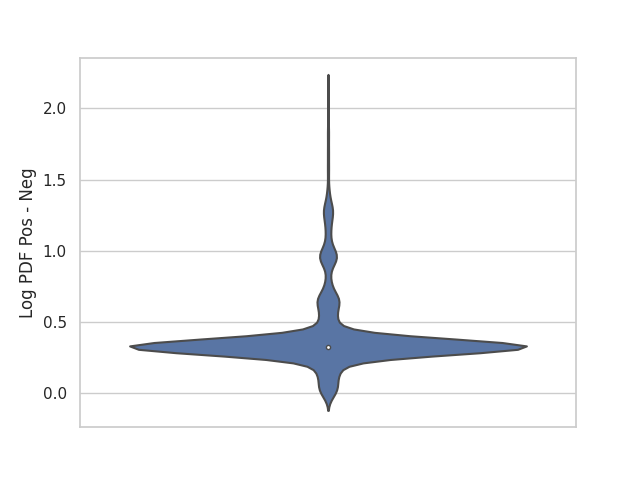
\includegraphics[trim=0cm 11mm 1cm 0pt, clip]{figures/analysis/embedprior/codex-s_analysis_prior_lpdf_diff.png}
        \caption{CoDEx-S}
    \end{subfigure}
    \begin{subfigure}[b]{0.492\columnwidth}
        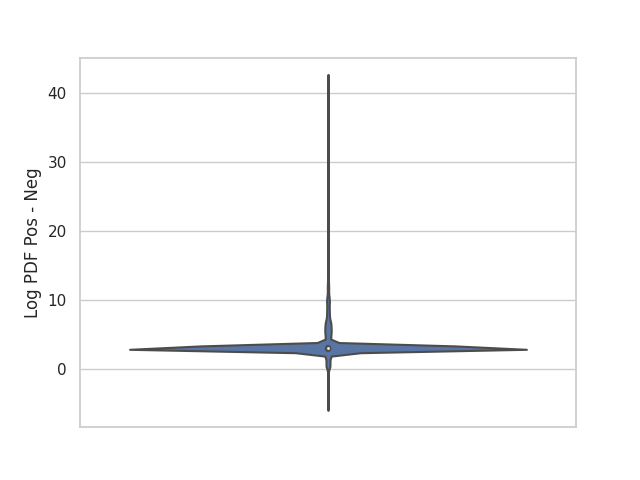
\includegraphics[trim=0cm 11mm 1cm 0pt, clip]{figures/analysis/embedprior/codex-m_analysis_prior_lpdf_diff.png}
        \caption{CoDEx-M}
    \end{subfigure}
    \vspace{-1em}
    \caption[Difference in density between positive and negative types.]{Difference in log-density between positive and negative types.}
    \label{fig:embedprior_lpdf_diffs}
\end{figure*}
However, as can be seen in Figure \ref{fig:embedprior_lpdf_diffs}, the actual difference in log-density that is obtained by the best performing checkpoint for each dataset does differ.
For FB15K-237 and WN18RR we can see that the constraint is satisfied for a lot of entities but not all. For the CoDEx datasets we can see that the constraint is violated for all entities.


\chapter{Conclusion \& Discussion}
\label{ch:conclusion}

% Answer the research question
% Refer back to motivation of work
% Then relate back to other work
% Highlight sections with most changes

% (RQ1) to what extent can type-information improve Link Prediction performance? and,
% (RQ2) what method of incorporating the type-information is most effective?

This chapter will outline the conclusions that may be drawn from the results of the experiments. They will be followed by some additional remarks, either detailing what else we may conclude from the results, or discussing how the results relate to previous investigations. 


\section*{Answering the Research Question}

%The central question we sought to answer in this thesis is as follows:
\begin{quote}
    \textit{(\textbf{RQ1})}
To what extent can type-information improve link-prediction performance? And,
\textit{(\textbf{RQ2})}
what method of incorporating the type-information is most effective?
\end{quote}
%
%By only embedding types instead of entities 
By embedding a type for each entity instead of the entity itself 
%\todo{rephrase? make clear that this is not to be taken too literally, the emphasis should be that entities of the same type do not have separate embeddings}%
-- which was an unintended effect of both the type-mean and type-attentive methods for some datasets -- we can get Link Prediction performance that is well beyond what seems possible otherwise. 
The improvement in MRR against the non-semantic baseline ranges from 261\% (for WN18RR) to 56\% (for CoDEx-M). 
From this we can conclude that type-information can greatly improve Link Prediction performance.

The second question asks what method is most effective.
When judged by our primary objective, which was Link Prediction performance, it is clear that for most datasets the type-attentive method is best. 
By representing entities by their most representative types, the method can exploit the type-information to obtain great Link Prediction performance.
The results on WN18RR, where the type-attentive-alt variant results in the highest MRR, shows that including the entity in the keys and values of the attention mechanism may yield even greater performance. Although the results of this method on the other datasets shows that this variant is less likely to find the low-entropy mode that makes the high MRR possible in the first place. If a way can be found to reliably find the low-entropy mode (see the Future Work section below) this variant may be superior.

\section*{Further Remarks}

\subsection{Additional Objectives}
In Section \ref{sec:method:objectives} we identified two additional objectives, the first of which was the ability to utilize Knowledge Graph Embeddings for downstream tasks. For that objective the type-attentive method seems less suited. For a lot of these tasks it is important that we actually learn a separate embedding for each entity, but as discussed previously, when the type-attentive method performs well it effectively only learns type-embeddings. 
Thus, despite a much more modest gain in MRR, the type-embedprior seems the better option when suitability for downstream tasks is important.

The other objective we identified was the ability to embed entities using their type(s) that were not seen during training. The type-mean can certainly do this, but that is all it can do, in essence it treats all entities as unseen entities, using only their type(s) for the embedding. Type-attentive still uses an entity representation to calculate the attention weights, so embedding unseen entities would be non-trivial. It might be possible to drop out the entity-specific representation during training so the model may learn to deal with this case effectively. 
Using the type-embedprior to embed unseen entities is also non-trivial, but for this method there is no mechanism at all to decide how to combine the distributions of the entity's types. Only if the unseen entity has just one type (or we know which is most representative) can we use the type-embedprior by simply sampling from that type's distribution.


\subsection{Comparing experimental results with \mycite{ma2017transt}}

In \cite{ma2017transt} TransT's performance for Link Prediction is tested on the outdated FB15K and WN18 datasets (see Section \ref{sec:method_type_linkprior}).
%
Furthermore, it is not clear that the baselines against which TransT was compared were run using the same experimental setup. From their code-base it seems that the baselines' performance came from previously reported numbers.

Both of these shortcomings are addressed in our experiments. We report the performance of the TransT configuration which \citeauthor{ma2017transt} refer to as `type information' (see Section \ref{sec:transt}).
We show that this method only outperforms the baseline on FB15K-237.
\citeauthor{ma2017transt} report an improvement in Mean Rank and Hits@10 on the WN18 dataset, we do not see the same for the WN18RR dataset.

%\todo{rho lower than what TransT paper set it}

\subsection{A prior on links: Type-linkprior(-only) vs. Type-attentive}

When the type-attentive model learns a low-entropy distribution over types -- effectively choosing one type per entity as the most-representative -- it no longer truly learns to embed entities, instead it only learns to embed types.
%
The type-linkprior and type-linkprior-only methods also do not try to incorporate type-information in entity-embeddings, but instead (re-)weigh the likelihood of triples being true.
%
However, of these two methods the type-attentive embedder is clearly the superior in terms of Link Prediction performance (see Table \ref{tab:hyperparam-search-results1}). If we wanted to model a type-based prior probability over links, then a separate KGE that uses the type-attentive embedder would be a far better choice than using the type-linkprior. 

%\subsection{}

\section*{Future Work}

\subsection{Taming the type-attentive[-alt] embedder}

In its current form, the type-attentive embedder is somewhat unpredictable, it exhibits substantially different behavior depending on whether it reached a low- or high-entropy mode (see Section \ref{sec:experiments:type_attentive}).
Say we want to use the type-attentive embedder in its low-entropy mode, then currently we have no way of making sure that this is what it learns.
Only when a particularly high learning rate is chosen for the attention mechanism does the model occasionally reach a well performing low-entropy state. 
%The same is true for the high-entropy mode, as it stands we are unable to study this mode for all datasets, because we cannot control when it finds the low-entropy or high-entropy modes.

The most obvious way to address this problem is to constrain the entropy of the distributions produced by the attention mechanism directly.
By doing this we can: produce high-entropy attention distributions to test if the originally intended behavior of the type-attentive embedder is useful; and produce low-entropy attention distributions to reliably reproduce the observed `most-representative type per entity' behavior.


\subsection{Combining type-attentive and type-embedprior}

Given the striking Link Prediction results of the type-mean and type-attentive models, it would make sense to explore ways of using their strengths while addressing their shortcomings. The main shortcoming of these methods is that they do not allow for learning of entity-specific embeddings. Instead they reduce the problem to learning only type-embeddings, and in the case of the type-attentive model, learning a most-representative type per entity.

To improve upon this we might take inspiration from the type-embedprior. It tries to learn both type-embeddings and entity-embeddings, the main intuition being that encouraging entities of the same type to be close to each other in the embedding space may be beneficial. However, in practice this resulted in only a modest improvement (see Section \ref{sec:experiments:results}).
It is possible that this is because there was not enough `signal' available for the type-distributions. This would explain why the added benefit we observe is so much less than that observed by \mycite{hao2019joie}, who supervise the type-embeddings with links from an ontology (meta-relations). 

Instead of using links from an ontology -- which are available only for select datasets -- we could use the regular links from the knowledge graph, using the type-attentive embedder to obtain a most-representative type per entity with which to translate entity-to-entity links into type-to-type links. These links could be used to supervise either the distances between the type-distributions' means $\mu$, or to supervise the type-distributions using distance metrics like those used by \mycite{he_learning_2015}.

Another version of this would forego the probabilistic aspect of the type-embeddings entirely. Thereby obtaining a method even closer to that of \citeauthor{hao2019joie} (the only difference being the use of links from the knowledge graph, rather than the ontology).


\subsection{Extending to other KGE methods}
Our experiments have been exclusively in combination with TransE. 
It will be useful to perform experiments in combination with other KGE methods. 
Investigating the generalization of our methodology to non-geometric KGE methods is of particular interest.
%\todo{OPTIONAL: finish. something about differences between geometric and tensor decomposition methods that could make it tricky to combine with the type-embedprior in particular}


\backmatter

\printbibliography
\newpage

\appendix

\renewcommand\thesection{\Alph{section}}
\renewcommand{\thetable}{\Alph{section}.\arabic{table}}

\chapter{Appendices}
\label{ch:appendices}

\clearpage
\section{Details hyper-parameter searches}
\label{apx:hyperparameter_search}


\subsection{Parameters - Training}
Like \citeauthor{ruffinelli_you_2019} we also use a learning rate schedule based on PyTorch's ReduceLROnPlateau class, with a reduction factor of 0.95, and a lower threshold of 0.0001.
Table \ref{tab:hyperparams-training} list the training hyper-parameters that were tuned, and the values that were considered.

\begin{table}[h!]
    \centering
    \begin{tabular}{lr}
        \toprule
        \textit{parameter}  & \textit{values}               \\
        \cmidrule{1-2}
        batch size          & 128, 256, 512, 1024              \\
        optimizer           & Adam, Adagrad                 \\
        learning rate (lr)  & [0.0001, 1.]                  \\
        lr schedule patience& [0, 10]                       \\
        \bottomrule
    \end{tabular}
    \label{tab:hyperparams-training}
    \caption{The hyper-parameters relating to the training process.}
\end{table}

\subsection{Parameters - Embeddings}
If a run uses `xavier\_normal' or `xavier\_uniform' the gain is always 1.0, if `normal' is used the mean is always 0.0 .
Table \ref{tab:hyperparams-embedding} list the embedding hyper-parameters that were tuned, and the values that were considered.

\begin{table}[h!]
    \centering
    \begin{tabular}{lr}
        \toprule
        \textit{parameter}              & \textit{values}                   \\
        \cmidrule{1-2}
        dimensions                      & 128, 256, 512                     \\
        initialization                  & xavier\_normal, xavier\_uniform,  \\
                                        & normal, uniform \\
        initialization.normal.std       & [0.00001, 1.0]                    \\
        initialization.uniform.a        & [-1.0, -0.00001]                  \\
        \cmidrule{1-2}
        regularization                  & none, l1, l2, l3                  \\
        regularization.weighted         & True, False                       \\
        regularization.weight $\dagger$ & [1.0e-20, 1.0e-01]                \\
        \cmidrule{1-2}
        dropout $\dagger$               & True, False                       \\
        dropout.prob $\dagger$          & [0.0, 0.5]                        \\
        \bottomrule
    \end{tabular}
    \label{tab:hyperparams-embedding}
    \caption[The hyper-parameters relating to the embeddings.]{The hyper-parameters relating to the embeddings. Parameters marked with a $\dagger$ are parameters that are set separately for each kind of embedding (entity, relation, type).}
\end{table}

\subsection{Parameters - TransE and negative-sampling}
We use a `shared' implementation of negative-sampling, meaning that the same negative samples are used for each triple in a batch. Note that it is ensured that a triple does not get itself as a negative.
Table \ref{tab:hyperparams-transe} list the TransE and negative-sampling hyper-parameters that were tuned, and the values that were considered.

\begin{table}[h!]
    \centering
    \begin{tabular}{lr}
        \toprule
        \textit{parameter}          & \textit{values}   \\
        \cmidrule{1-2}
        l-norm                      & 1.0, 2.0          \\
        normalize.p $\dagger$       & None, 2.0  \\
        \cmidrule{1-2}
        num-negative-samples.s      & [1, 1000] \\
        num-negative-samples.o      & [1, 1000] \\
        \bottomrule
    \end{tabular}
    \vspace{1cm}
    \label{tab:hyperparams-transe}
    \caption[The hyper-parameters relating to TransE and negative sampling.]{The hyper-parameters relating to TransE and negative sampling. Parameters marked with a $\dagger$ are parameters that are set separately for each kind of embedding (entity, relation, type).}
\end{table}

\subsection{Parameters - Type-linkprior}
Table \ref{tab:hyperparams-linkprior} list the Type-linkprior hyper-parameters that were tuned, and the values that were considered.
\begin{table}[h!]
    \centering
    \begin{tabular}{lr}
        \toprule
        \textit{parameter}          & \textit{values}   \\
        \cmidrule{1-2}
        $\lambda_{head}$            & [0.0, 1.0]        \\
        $\lambda_{relation}$        & [0.0, 1.0]        \\
        $\lambda_{tail}$            & [0.0, 1.0]        \\
        $\rho$                      & [0.0, 1.0]        \\
        learn-$\lambda$             & True, False       \\
        \bottomrule
    \end{tabular}
    \label{tab:hyperparams-linkprior}
    \caption[The hyper-parameters relating to the Type-linkprior method.]{The hyper-parameters relating to the Type-linkprior method. }
\end{table}



\subsection{Parameters - Type-mean}
The only hyper-parameter specific to the type-mean methods is the `use\_entity\_embedder' that determines if we are using the entity-specific offsets as described in \ref{sec:methods:type_mean}. 


\subsection{Parameters - Type-attentive}
Table \ref{tab:hyperparams-attentive} list the Type-attentive hyper-parameters that were tuned, and the values that were considered.
\begin{table}[h!]
    \centering
    \begin{tabular}{lr}
        \toprule
        \textit{parameter}                & \textit{values}   \\
        \cmidrule{1-2}
        type\_attn\_nr\_heads              & 1, 2, 4, 8        \\
        type\_attn\_lr                    & [0.0001, 1.0]     \\
        \cmidrule{1-2}
        mutual\_information\_min          & [-20.0, 20.0]%
        \tablefootnote{Negative values disable the mutual information constraint.}       \\
        mutual\_information\_min\_scale   & [0.01, 100.0]      \\
        mutual\_information\_min\_damping & [0.01, 100.0]      \\
        \bottomrule
    \end{tabular}
    \label{tab:hyperparams-attentive}
    \caption[The hyper-parameters relating to the Type-attentive method.]{The hyper-parameters relating to the Type-attentive method. }
\end{table}



\subsection{Parameters - Type-embedprior}
Table \ref{tab:hyperparams-embedprior} list the Type-attentive hyper-parameters that were tuned, and the values that were considered.
\begin{table}[h!]
    \centering
    \begin{tabular}{lr}
        \toprule
        \textit{parameter}          & \textit{values}   \\
        \cmidrule{1-2}
        type\_prior\_init\_std         & [0.0, 1.0]     \\
        type\_nll\_min              & [-20.0, 0.0]      \\
%        type\_nll\_min\_scale       & [0.01, 100.0]     \\
%        type\_nll\_min\_damping     & [0.01, 100.0]     \\
        \bottomrule
    \end{tabular}
    \label{tab:hyperparams-embedprior}
    \caption[The hyper-parameters relating to the Type-embedprior method.]{The hyper-parameters relating to the Type-embedprior method.}
\end{table}



\newpage
\section{Additional performance metrics of hyper-parameter search}
\setcounter{table}{0}
\begin{table}
    \def\fn{\hspace{2pt}} % footnote columns
    \setlength{\tabcolsep}{5pt}
    \centering
    \begin{tabular}{lr@{\fn}lr@{\fn}lr@{\fn}lr@{\fn}l}
        \toprule
        \textit{name}
                &\multicolumn{2}{c}{WN18RR}
                            &\multicolumn{2}{c}{FB15K-237}   
                                           & \multicolumn{2}{c}{CoDEx-S}   
                                                                & \multicolumn{2}{c}{CoDEx-M} \\
        \cmidrule{1-9}
        non-semantic         &  5.24    && {21.37}  && 21.13    && 22.14  \\
        \cmidrule{1-9}
        type-linkprior-only  & 00.00    &&  9.58	&&  3.09    &&  3.29   \\
        type-linkprior       &  1.17	&& 23.06    && 23.81    && 19.72    \\
        \cmidrule{1-9}
        type-mean            & 72.33    && 23.31    && 35.74    && 30.11  \\
        type-mean+           &  5.19    && 23.31    && 23.56    && 19.68  \\
        type-attentive       & -        && \textbf{61.44}    
                                                    && \textbf{45.87}     
                                                                && \textbf{44.79}  \\
        type-attentive-alt   & \textbf{81.05} 
                                        && 21.13    && 22.03    && 41.35  \\
        \cmidrule{1-9}
        type-embedprior      &  6.38    && 22.57    && 25.42    && 21.68  \\
        \bottomrule
    \end{tabular} \vspace{1em}
    \caption[Hits@1 obtained by each method for best set of hyperparameters.]{Hits@1 (\%) obtained by each method for best set of hyperparameters. }\label{tab:hyperparam-search-results3a}
\end{table}

\begin{table}
    \def\fn{\hspace{2pt}} % footnote columns
    \setlength{\tabcolsep}{5pt}
    \centering
    \begin{tabular}{lr@{\fn}lr@{\fn}lr@{\fn}lr@{\fn}l}
        \toprule
        \textit{name}
                &\multicolumn{2}{c}{WN18RR}
                            &\multicolumn{2}{c}{FB15K-237}   
                                           & \multicolumn{2}{c}{CoDEx-S}   
                                                                & \multicolumn{2}{c}{CoDEx-M} \\
        \cmidrule{1-9}
        non-semantic         & 36.01    && 34.23
                                                    && 42.88    && 34.27  \\
        \cmidrule{1-9}
        type-linkprior-only  & 00.00    && 14.98	&& 11.77    &&  4.78  \\
        type-linkprior       & 35.78	&& 35.73    && 40.07    && 32.37  \\
        \cmidrule{1-9}
        type-mean            & 72.33    && 29.29    && 47.13    && 37.21  \\
        type-mean+           & 23.88    && 34.90    && 39.60    && 30.67  \\
        type-attentive       & -        && \textbf{61.44}    
                                                    && \textbf{75.18}     
                                                                && 46.86  \\
        type-attentive-alt   & \textbf{82.22} 
                                        && 32.79    && 38.81    && \textbf{46.99}  \\
        \cmidrule{1-9}
        type-embedprior      & 40.05    && 34.92    && 43.43    && 33.43  \\
        \bottomrule
    \end{tabular} \vspace{1em}
    \caption[Hits@3 obtained by each method for best set of hyperparameters.]{Hits@3 (\%) obtained by each method for best set of hyperparameters. }\label{tab:hyperparam-search-results3b}
\end{table}



\listoftodos

\printindex

\end{document}
